\chapter{Anharmonic Phonons with Gaussian Processes} \label{ch:3}

\paragraph{}
%In this chapter, we explore the extension of differentiable Gaussian process models and their application to the prediction of harmonic (FC2) and cubic anharmonic (FC3) force constants. We present the development and implementation of \textsc{GPFC.jl}, a Julia package designed to facilitate this approach.

In this chapter, we introduce an approach for predicting harmonic (FC2) and cubic anharmonic (FC3) force constants using differentiable Gaussian process (GP) models.
This approach uses the smoothness and uncertainty quantification offered by GPs to efficiently estimate force constants from a small number of atomic configurations.
We describe how this methodology is implemented in the \textsc{GPFC.jl} package and show how it may be used for calculations involving phonons and lattice dynamics.
%We will start the discussion from the relation between the force constants and  differentiable GP models, how this relation can be used to construct the formulations for predicting FC2 and FC3, the results and their discussions.

We begin by establishing the connection between force constants and differentiable Gaussian process (GP) models. Building on this foundation, we derive the formulation of a derivative GP model using Cartesian descriptors for predicting harmonic (FC2) and cubic anharmonic (FC3) force constants. The results and discussions are presented in Section~\ref{sec:3.1}.
Section~\ref{sec:3.2} introduces the use of phonon descriptors in \textsc{GPFC.jl}. 
These descriptors naturally impose translational symmetry and reduce the model size, leading to an improvement in the accuracy and efficiency of the model.  
We compare the learning behaviour of models trained with phonon descriptors versus Cartesian descriptors and outline the procedure for recovering FC2s and FC3s from the phonon basis to the Cartesian basis.
Section~\ref{sec:3.3} discusses possible extensions, including the integration of atomic cluster expansion (ACE) descriptors and the use of active learning strategies for enlarging training sets, facilitated by \textsc{ACEpotentials.jl}.
Finally, Section~\ref{sec:3.4} outlines directions for future work.


%In this chapter, we present a framework for predicting harmonic (FC2) and cubic anharmonic (FC3) force constants using differentiable Gaussian process (GP) models. This approach enables efficient estimation of force constants from a limited number of atomic configurations by leveraging the smoothness and uncertainty quantification provided by GPs. We detail the implementation of this methodology in the \texttt{GPFC.jl} package, and demonstrate its applicability to lattice dynamics and phonon-related calculations.

%the mathematical details and algorithm of a GP model for calculating the second and third order force constants (FC) of an atomic environment by training the model on its input potential energies and its force fields. Accordingly, a \textit{square exponential} GP \textit{kernel} is defined in the first section. In the following section (\ref{sec:3.2}), the exact forms of kernel derivatives (from the first to fourth order) are shown through full derivation, while the full derivation of the fifth and sixth order is served in appendix \ref{c:A}. Obtaining these derivatives allows us to use the prior energies and forces to calculate the posterior second and third order FCs through the algorithm provided in section \ref{sec:3.3}.

\section{\textsc{GPFC.jl} with Cartesian descriptors} \label{sec:3.1}
\paragraph{}
In this section, we describe the construction of the differentiable Gaussian process (GP) model used in \textsc{GPFC.jl} for predicting force constants from atomic forces, using Cartesian descriptors.
Cartesian descriptors represent atomic environments directly in terms of relative atomic positions, preserving full spatial resolution without imposing any symmetry constraints.
This choice allows us to directly construct the GP model derivatives with respect to atomic displacements, enabling the prediction of harmonic and cubic anharmonic force constants (FC2s and FC3s) from prior energies and forces of materials.
We begin by outlining the theoretical formulation of the GP model and its derivatives, followed by implementation details and validation results.

\subsection{Higher Derivative GP Model} \label{subsec:3.1.1}

To extract harmonic and anharmonic force constants from a derivative Gaussian process (GP) model of the force field, it is necessary to compute higher-order derivatives of the predicted forces with respect to atomic displacements. Specifically, the second derivatives correspond to the force constant matrix (FC2), and the third derivatives yield the cubic anharmonic force constants (FC3), as defined in the Taylor expansion of the potential energy in Equation~\eqref{equ:2.2}. 

We begin by revisiting the derivative GP model with a kernel function $k(\mathbf{x},\mathbf{x}^{*})$ which defines the similarity between the descriptor $\mathbf{x}$ and $\mathbf{x}^{*}$ of $N$ atoms in Cartesian representations, i.e. $\mathbf{x},\;\mathbf{x}^{*}\in\mathbb{R}^{3N}$.
In our implementation, we mainly use the square exponential (radial basis function: RBF) kernel, equivalent to \eqref{equ:2.32}, generically defined as
\begin{equation} \label{equ:3.1}
        \begin{split}
            k(\mathbf{x},\;\mathbf{x}^{*})= \sigma_{o}\mathbf{exp}\left[-\frac{1}{2\ell^{2}}d(\mathbf{x},\;\mathbf{x}^{*})^{2}\right],
        \end{split}
\end{equation}
where $d(\mathbf{x},\;\mathbf{x}^{*})=\lVert\mathbf{x}-\mathbf{x}^{*}\rVert^{2}_{2}$ is the Euclidean metric.
The kernel scale $\sigma_{o}$ and the length scale $\ell$ can be obtained from the hyperparameter optimisation.

The SE kernel was chosen because it assumes a smooth, infinitely differentiable latent function. This is physically well-motivated for electronic-structure-related quantities like potential energies that change smoothly with small changes in geometry. 
Its isotropic form also provides a straightforward way to encode geometric similarity without introducing additional directional parameters, making it computationally efficient and numerically stable during training.

A systematic grid-based scan was used to find the kernel hyperparameters $\sigma_{0}$ and $\ell$ instead of doing full evidence maximisation. 
This manual optimisation method was used to make sure that the smoothness and amplitude scales were under control. This way, the chosen values would match the physically meaningful changes in the data without causing numerical problems that can happen when automatic optimisation is used on small or noise-sensitive datasets.

Conditioning this GP model with the energy $E$ and forces $\nabla E$ at $\mathbf{x}$ yields the posterior potential energy at $\mathbf{x}^{*}$, analogous to \eqref{equ:2.44} and \eqref{equ:2.51}, expressed as
\begin{equation} \label{equ:3.2}
        E(\mathbf{x}^{*}) = 
        \begin{bmatrix}
              k & (\nabla_{\mathbf{x}} k)^{\textbf{T}}
        \end{bmatrix}_{\textbf{x},\textbf{x}^{*}}
        \cdot \mathcal{K}^{-1}_{\mathbf{x},\: \mathbf{x}}
        \cdot
        \begin{bmatrix}
              E \\
              \nabla E
        \end{bmatrix}_{\mathbf{x}},
\end{equation}
where the subscripts indicate the functions evaluated at the descriptors.
The first derivative of the kernel function $(\nabla_{\mathbf{x}} k)$ with respect to the descriptor $\mathbf{x}$ correlates the potential energy at $\mathbf{x}^{*}$ to the force fields at $\mathbf{x}$.
This derivative, as mentioned in section \ref{subsec:2.3.2}, can be represented as a $3N\times1$ covariance matrix (Jacobian matrix as a first rank tensor)
\begin{equation} \label{equ:3.3}
    \left[\nabla_{\mathbf{x}}
    k(\mathbf{x},\:\mathbf{x}^{*})\right]^{\textbf{T}}
    = \left[\frac{\partial k}{\partial x_{1}}\ \ \frac{\partial k}{\partial x_{2}}\cdots\frac{\partial k}{\partial x_{3N}} \right]^{\textbf{T}}.
\end{equation}
Marginal likelihood covariance matrix $\mathcal{K}$ which defines the probability distribution $(1+3N)\times(1+3N)$ matrix of the priors, is 
\begin{equation} \label{equ:3.4}
\mathcal{K}(\mathbf{x},\: \mathbf{x}) = 
\begin{bmatrix}
             k & (\nabla_{\mathbf{x}} k)^{\textbf{T}}\\
             \nabla_{\mathbf{x}^{*}} k & \nabla_{\mathbf{x}^{*}}\nabla_{\mathbf{x}} k
\end{bmatrix}_{\mathbf{x},\: \mathbf{x}}
+
\begin{bmatrix}
             \sigma^{2}_{e} & \mathbf{0}\\
             \mathbf{0} & \sigma^{2}_{f}\cdot\mathbb{1}_{3N\times 3N}
\end{bmatrix}.
\end{equation}
The first matrix contains the \textbf{kernel}, the \textbf{Gradient kernel}, and the \textbf{Hessian kernel} for constructing the correlation between the prior energy and the prior forces.
The expressions of those derivatives of the kernel functions are illustrated in \eqref{equ:3.3} and \eqref{equ:2.40}.
The second matrix is the observation noise matrix, which includes $\sigma_{e}$ and $\sigma_{f}$ indicates observation noises for prior energy and force, respectively.
One of the choices for these noises is the energy and force convergence factor in the underlying electronic structure calculations used for training.

The recent works \cite{GarijodelRo2019, Kaappa2021, Asnaashari2021, Deringer2021} on the derivative GPs suggested that the prediction of potential energy can be potentially extended to predict forces at $\mathbf{x}^{*}$.
This force prediction requires evaluating the first and second order derivatives of the kernel function with respect to $\mathbf{x}$ and $\mathbf{x}^{*}$ as follows:
\[\nabla_{\mathbf{x}^{*}} k \quad \text{and}\quad \nabla_{\mathbf{x}^{*}}\nabla_{\mathbf{x}} k.
\]
The first derivative is already expressed in Equation \eqref{equ:2.39}.
The second derivative is defined as the $(3N\times 3N)$ rank-2 tensor, linking the force fields at $\mathbf{x}$ to the force fields at $\mathbf{x}^{*}$.
This allows us to reconstruct \eqref{equ:3.2} with changes in those covariance matrices:
\begin{equation} \label{equ:3.5}
        \nabla E(\mathbf{x}^{*}) = 
        \begin{bmatrix}
             \nabla_{\mathbf{x}^{*}} k & \nabla_{\mathbf{x}^{*}}\nabla_{\mathbf{x}} k
        \end{bmatrix}_{\textbf{x}^{*},\textbf{x}}
        \cdot \mathcal{K}^{-1}_{\mathbf{x},\: \mathbf{x}}
        \cdot
        \begin{bmatrix}
              E \\
              \nabla E
        \end{bmatrix}_{\mathbf{x}}.
\end{equation}

Motivated by this extension, we perform the higher-order differentiation to predict the harmonic (FC2) and cubic anharmonic (FC3) force constants and present the model construction in our work \cite{https://doi.org/10.48550/arxiv.2405.05113}.
To predict FC2 requires extra differentiation on those covariance matrices with respect to $\mathbf{x}^{*}$ which are equivalent to the second and third order kernel derivative with respect to $\mathbf{x}$ and $\mathbf{x}^{*}$, given by
\begin{equation} \label{equ:3.6}
    (\nabla_{\mathbf{x}^{*}})^{2} k \quad \text{and}\quad (\nabla_{\mathbf{x}^{*}})^{2}  \nabla_{\mathbf{x}} k.
\end{equation}
These $(3N\times 3N)$ rank-2 and $(3N\times 3N\times 3N)$ rank-3 tensors are interpreted as the covariance correlating the harmonic force constant at $\mathbf{x}^{*}$ to the energy and to the forces, respectively at $\mathbf{x}$.
Equation \eqref{equ:3.5} can, then, be modified into 
\begin{tcolorbox}[
    ams equation,
    title=GPFC2 prediction,
    %colback=blue!5,
    colframe=bEpic,
    %colframe=blue!75!black,
    coltitle=white,
    %fontupper=\color{blue}  % << changes font color inside the box
]
\label{equ:3.7}
\begin{split}
    \Phi^{(2)}(\mathbf{x}^{*}) = 
    \begin{bmatrix}
          (\nabla_{\mathbf{x}^{*}})^2 k &
          (\nabla_{\mathbf{x}^{*}})^2 \nabla_{\mathbf{x}} k
    \end{bmatrix}_{\textbf{x},\;\textbf{x}^{*}}
        \cdot \mathcal{K}^{-1}_{\mathbf{x},\: \mathbf{x}}
        \cdot
        \begin{bmatrix}
              E \\
              \nabla E
        \end{bmatrix}_{\mathbf{x}},
\end{split}
\end{tcolorbox}
where $\Phi^{(2)}$ is the Gaussian process $(3N\times 3N)$ harmonic force constant tensor (GPFC2) at descriptor $\mathbf{x}^{*}$, constructed by correlating all degrees of freedom of $\mathbf{x}^{*}$ via the derivative GP model.

It is important to emphasise that this formulation follows the same fundamental learning framework as the original Gaussian Approximation Potential (GAP) approach~\cite{Bartk2010}, which already incorporates total energy and derivative (force) observations as training targets, combined with sparsification for computational efficiency. 
As reviewed comprehensively in \textit{Chemical Reviews} (2021)~\cite{Deringer2021}, this joint energy–force learning strategy underpins nearly all GAP-based applications to molecular and condensed-phase systems. 
The present Gaussian Process Force Constant (GPFC) model adopts this established foundation but extends it through an additional analytical differentiation of the trained Gaussian process posterior, allowing direct computation of higher-order force constants (harmonic and cubic anharmonic) from the same learned potential energy surface.

This post-processing differentiation step—absent from the original GAP formalism—constitutes the principal methodological novelty of the GPFC framework.

Equation~\eqref{equ:3.7} can be constructed as a tensor contraction (instead of the matrix multiplication) as illustrated in Figure~\ref{fig:3.1}a. The resulting harmonic force constant tensor $\Phi^{(2)}$ is predicted at descriptor $\mathbf{x}^{*}$, as shown in Figure~\ref{fig:3.1}b, for a $2 \times 1 \times 1$ diamond-structure silicon supercell depicted in Figure~\ref{fig:3.1}c~\cite{https://doi.org/10.48550/arxiv.2405.05113}.

\begin{figure*}[t]
\centering
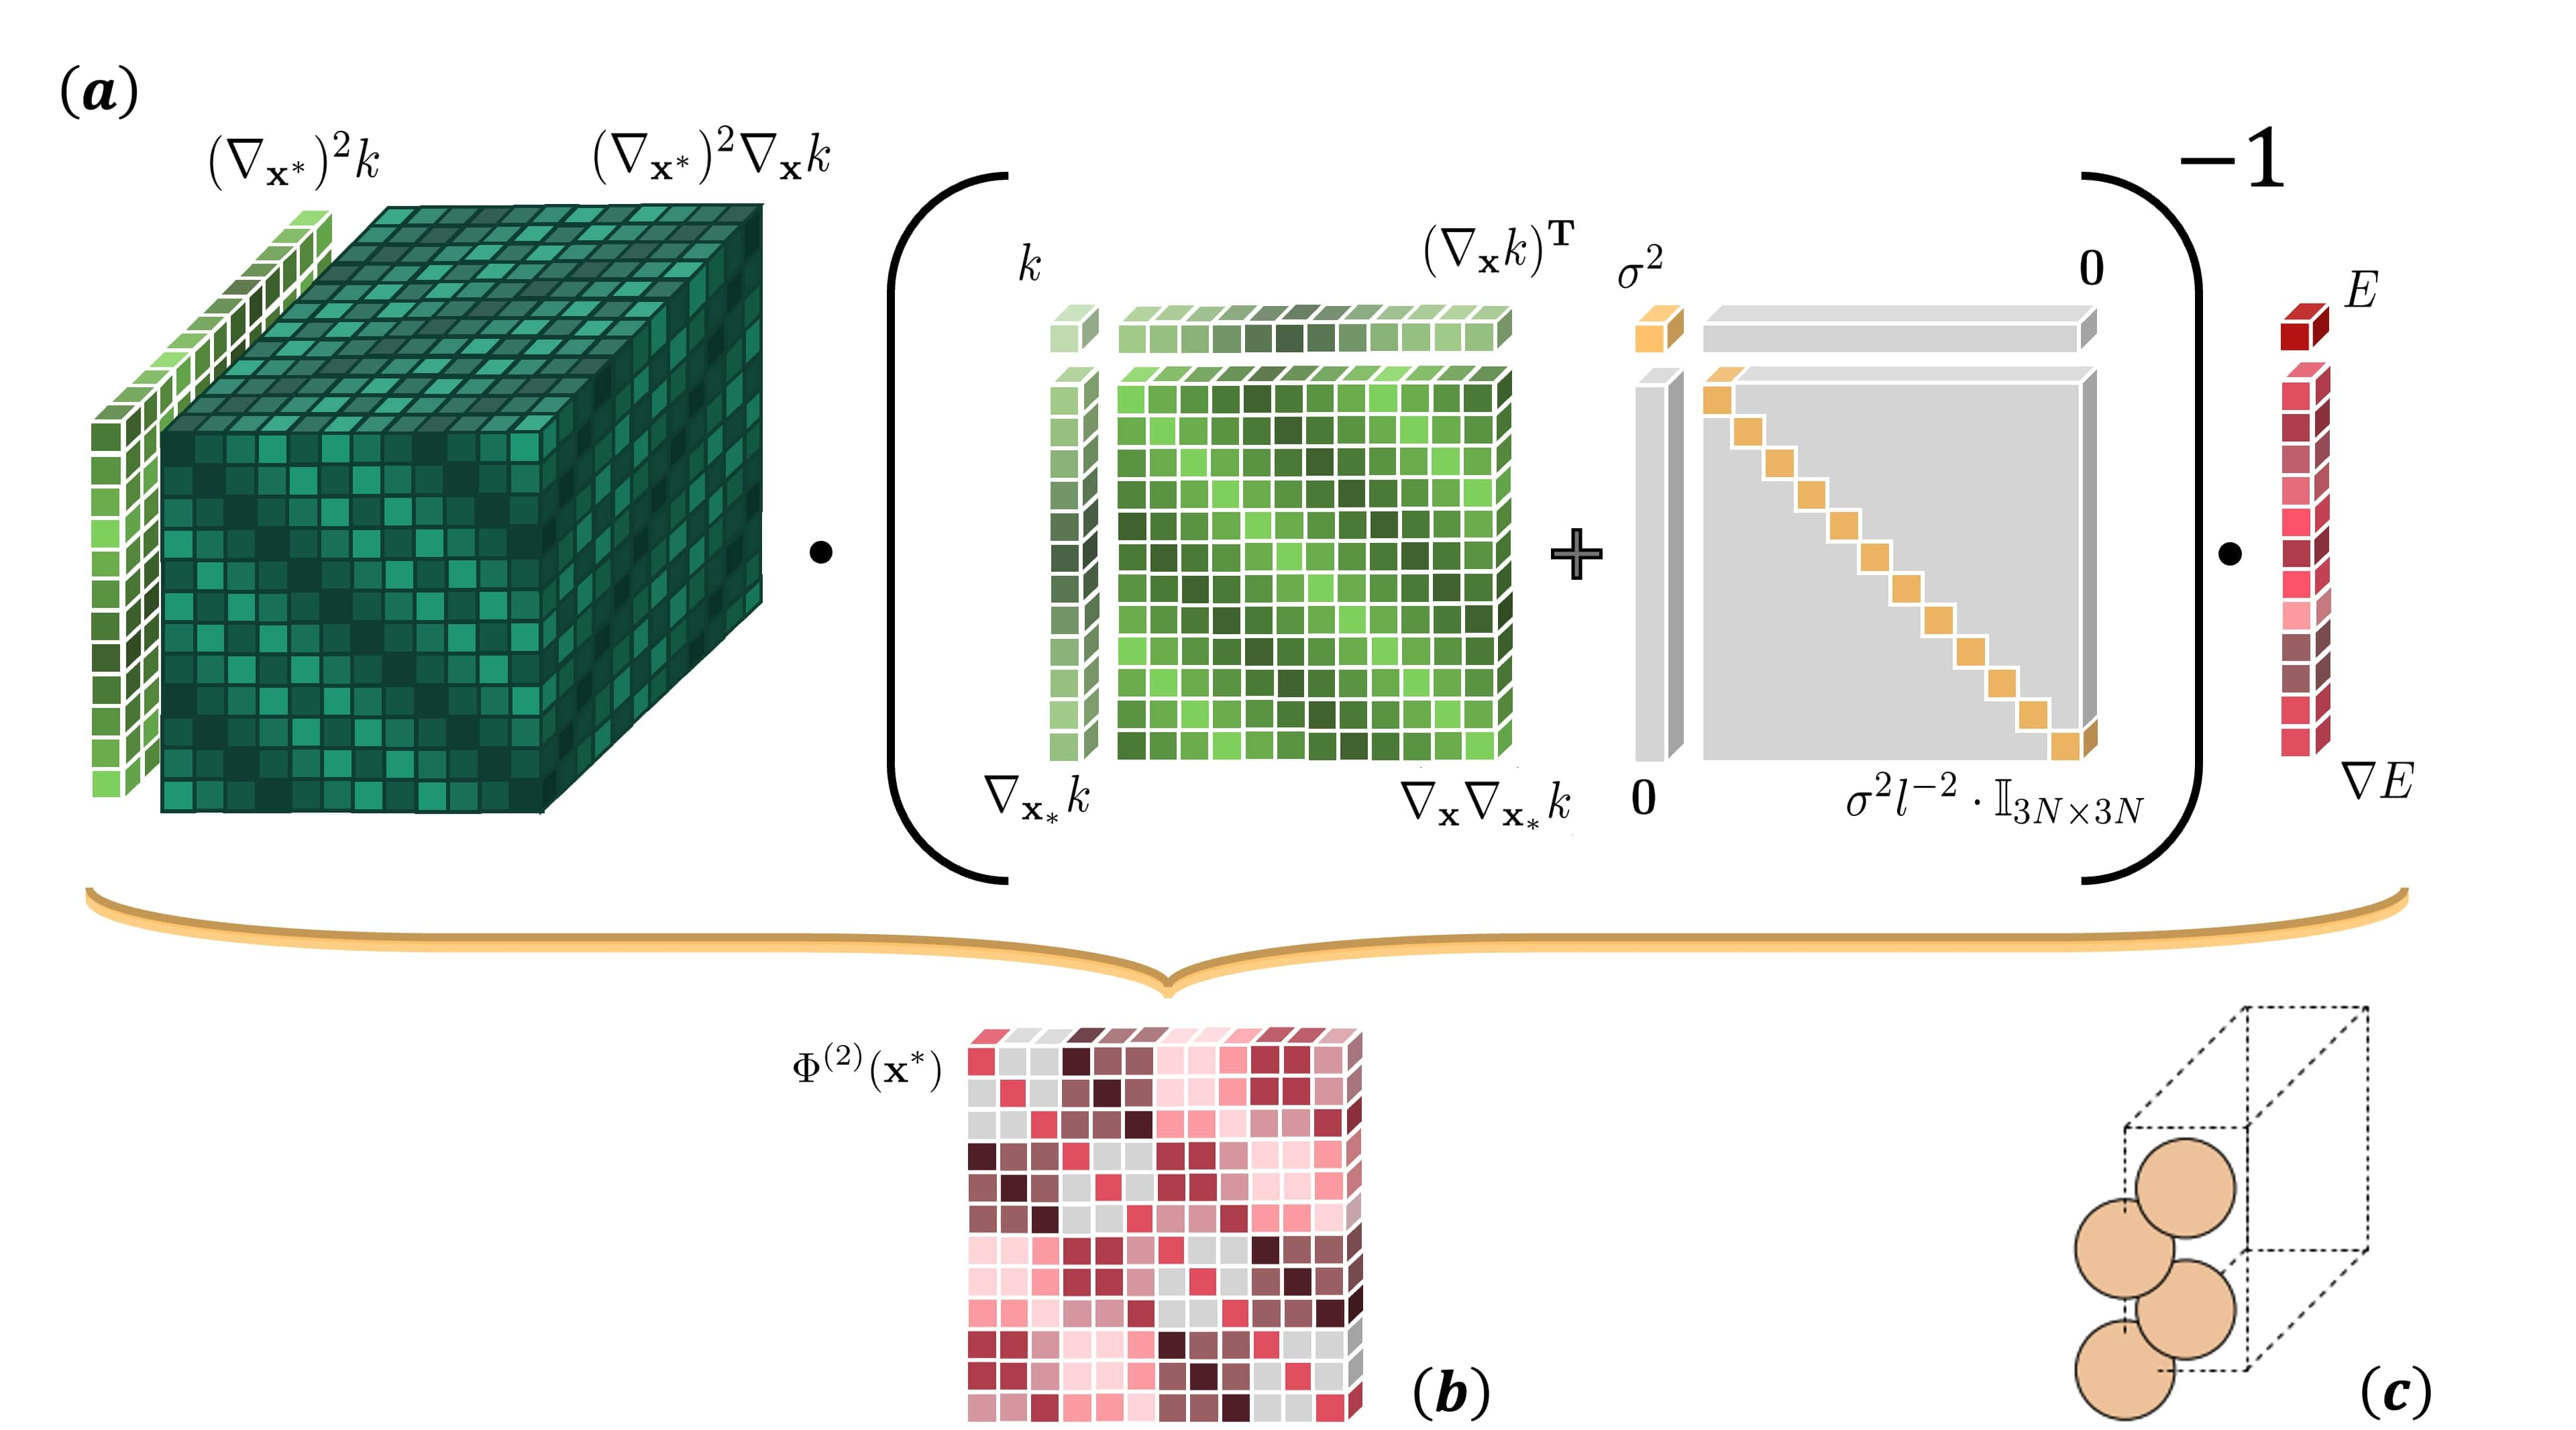
\includegraphics[width=1.0\textwidth]{Figure/Chapter 3/GPFC_cart.jpg}
\caption{\label{fig:3.1} Figure%~(3.1a)
illustrates the tensor contraction in Equation~\eqref{equ:3.7}, where the derivative GP model is trained on a single data point at descriptor $\mathbf{x}$. 
%The resulting harmonic force constant tensor $\Phi^{(2)}$ is predicted at descriptor $\mathbf{x}^{*}$, as shown in Figure~(3.1b), for a $2 \times 1 \times 1$ diamond-structure silicon supercell depicted in Figure~(3.1c)~\cite{https://doi.org/10.48550/arxiv.2405.05113}.
}
\end{figure*}

The prediction of the cubic anharmonic force constant (FC3), similarly, requires evaluating the rank-3 and rank-4 covariance tensors correlating the FC3 to the potential energy and to the force fields, respectively.
These covariance tensors are defined as
\begin{equation} \label{equ:3.8}
    (\nabla_{\mathbf{x}^{*}})^{3} k \quad \text{and} \quad (\nabla_{\mathbf{x}^{*}})^{3} \nabla_{\mathbf{x}} k.
\end{equation}
Evaluating these allows us to recast Equation \eqref{equ:3.7} as
\begin{tcolorbox}[
    ams equation,
    title=GPFC3 prediction,
    %colback=blue!5,
    colframe=bEpic,
    %colframe=blue!75!black,
    coltitle=white,
    %fontupper=\color{blue}  % << changes font color inside the box
]
\label{equ:3.9}
\begin{split}
    \Phi^{(3)}(\mathbf{x}^{*}) = 
    \begin{bmatrix}
          (\nabla_{\mathbf{x}^{*}})^3 k &
          (\nabla_{\mathbf{x}^{*}})^3 \nabla_{\mathbf{x}} k
    \end{bmatrix}_{\textbf{x},\;\textbf{x}^{*}}
        \cdot \mathcal{K}^{-1}_{\mathbf{x},\: \mathbf{x}}
        \cdot
        \begin{bmatrix}
              E \\
              \nabla E
        \end{bmatrix}_{\mathbf{x}},
\end{split}
\end{tcolorbox}
where $\Phi^{(3)}$ the predicted cubic anharmonic force constant tensor (GPFC3) is the size of $(3N\times 3N\times 3N)$.

With these methods for directly evaluating force constants from the fitted Gaussian process model, we now have all the essential components for performing lattice dynamics calculations, including anharmonic effects.

\begin{figure*}[t]
  \centering
  \begin{lstlisting}[language=Julia]
using KernelFunctions       # Kernel methods for ML
using ForwardDiff           # Forward-mode AD 
using Zygote                # Reverse-mode AD

kernel = SqExponentialKernel()  # Define RBF kernel

function diff3_kernel(kernel, x, x_star)
    ForwardDiff.(*@\textcolor{bEpic}{jacobian}@*)(
        a -> Zygote.(*@\textcolor{bEpic}{hessian}@*)(
            b -> kernel(b, x_star),
            a
        ),
        x
    )
end
  \end{lstlisting}
  \caption{\label{fig:3.2} Julia implementation of a third-order derivative of a kernel function, computed by applying forward-mode automatic differentiation (AD) via \texttt{ForwardDiff.jacobian} on the Hessian obtained from reverse-mode AD via \texttt{Zygote.hessian}. %The example uses a squared exponential (RBF) kernel from \texttt{KernelFunctions.jl}.
  }
\end{figure*}

To efficiently evaluate those derivatives of the kernel function, our implementation employs \textsc{ForwardDiff.jl} and \textsc{Zygote.jl}, \textit{Automatic Differentiation (AD)} packages in \textsc{Julia}, for doing differentiation on the kernel function defined from \textsc{KernelFunctions.jl}.
The example of the evaluation of the third-order derivative of the square exponential kernel with respect to $\mathbf{x}$, $(\nabla_{\mathbf{x}})^{3}k$, is given by the code in Figure \ref{fig:3.2}.

Combining these two AD packages results in the efficient computation of higher-order derivatives compared to implementing \textsc{ForwardDiff.jl} purely. 
This is due to the fact that \textsc{Zygote.jl}'s reverse-mode AD effectively manages scalar-output functions with substantially reduced memory allocations, avoiding the computational cost of repeating nested forward-mode dual number evaluations, which are necessary for higher-order derivatives.

Moreover, the full derivations for differentiating the kernel function to arbitrary order with respect to the input descriptors are provided in Appendix~\ref{sec:A.1}. These derivations reveal the symmetry and antisymmetry properties of derivative kernels in \eqref{equ:3.6} and \eqref{equ:3.8}, at a given order, which can be exploited to significantly reduce the number of required kernel derivative evaluations.


\subsection{Dataset Preparation \& Training} \label{subsec:3.1.2}

To evaluate the performance of our method and compare it with standard approaches, we consider a set of representative solid-state materials. We benchmark our approach—referred to as GPFC (Gaussian Process Force Constants)—against two established methods: the traditional finite displacement method, as implemented in \textsc{Phonopy}~\cite{phonopy,Phonopy_toolkit}, and third-order many-body perturbation theory, as implemented in \textsc{Phono3py}~\cite{Togo2015-qf,Phonopy_toolkit}. For consistency and comparability, we process force constants predicted by our model using both \textsc{Phonopy} and \textsc{Phono3py}.
\subsubsection{Dataset Preparation}
Details of the training datasets used for each method are provided below:
\begin{itemize}
    \item \textbf{\textsc{phono(3)py}-dataset}: We use the \textsc{phono(3)py} package to generate displaced structures of $2 \times 2 \times 2$ supercells using the finite difference method (FDM). Energies and forces for these structures are computed using density functional theory (DFT) via \textsc{VASP}, with the following parameters: plane-wave cutoff energy (\textsc{ENMAX} = 800 eV), self-consistent field energy convergence (\textsc{EDIFF} = $10^{-8}$ eV), and a Monkhorst–Pack $k$-point mesh of $[6, 6, 6]$. The resulting forces are processed with \textsc{Phonopy} to generate FC2s and FC3s using space group symmetry operations.
    \item \textbf{\textsc{GPFC}-dataset}: Rattled $2 \times 2 \times 2$ supercell structures are generated using the \textsc{ASE} package, with random displacements sampled from a normal distribution with a standard deviation of $0.01$~\AA. Using the same computational parameters earlier mentioned, DFT is used in \textsc{VASP} to calculate the corresponding energies and forces.  Equations~\eqref{equ:3.5} and~\eqref{equ:3.6} describe how the derivative GP model is trained using these data without imposing any symmetry constraints.
\end{itemize}
\subsubsection{Training}
In the training process, we aim to optimise the hyperparameters of the GPFC model—namely, the kernel output scale $\sigma_{o}$, the length scale $l$, and the observation noise parameters for the potential energy $\sigma_{e}$ and forces $\sigma_{f}$—by maximising the logarithm of the marginal likelihood of the prior dataset.

Let the prior dataset consist of $m$ total-energy values and corresponding force vectors, each associated with a descriptor $\mathbf{x}_i$ for a "global" system of $N$ atoms. We denote
\begin{subequations}
\begin{align} 
   \label{equ:3.10a} 
   \mathbf{E} &:= \left[E_{1}\:E_{2}\cdots E_{m} \right]^{\text{T}},\\
   \label{equ:3.10b} 
   \mathbf{f} &:= \left\{\nabla_{\mathbf{x}_{1}} E_{1}\:\nabla_{\mathbf{x}_{2}} E_{2}\cdots \nabla_{\mathbf{x}_{m}} E_{m} \right\},\\
   \label{equ:3.10c} 
   \mathbf{X} &:= \left\{\mathbf{x}_{1},\, \mathbf{x}_{2},\, \cdots,\, \mathbf{x}_{m} \right\},
\end{align}
\end{subequations}

where $\mathbf{E}$ and $\mathbf{f}$ represent the training targets for energy and force, respectively.
Each energy $E_i$ is subject to observation noise $\sigma_{e}$ arising from electronic structure calculation errors or convergence limitations and can be expressed as:
\begin{equation}
    \label{equ:3.11}
E_{i} = E(\mathbf{x}_{i}) + \epsilon_{e}, \quad \epsilon_{e} \sim \mathcal{N}(0,\;\sigma_{e}^{2}).
\end{equation}
Similarly, each force vector $\nabla_{\mathbf{x}_{i}} E_i$ carries its own observation noise $\sigma_{f}$:
\begin{equation}
    \label{equ:3.12}
\nabla_{\mathbf{x}_{i}} E_{i} = \nabla_{\mathbf{x}_{i}} E(\mathbf{x}_{i}) + \boldsymbol\epsilon_{f}, \quad \boldsymbol\epsilon_{f} \sim \mathcal{N}_{3N}(\mathbf{0},\;\Sigma_{f} ),
\end{equation}
where $\Sigma_{f} = \sigma^{2}_{f}\cdot\mathbb{1}_{3N\times 3N}$.

Assuming \eqref{equ:3.11} and \eqref{equ:3.12} allows us to construct an independent $(1+3N)$-multivariate distribution for a pair $\mathbf{y}_{i}$ of the energy $E_{i}$ and the corresponding force fields $\nabla_{\mathbf{x}_{i}} E_{i}$, i.e., 
\[\mathbf{y}_{i}=\begin{bmatrix}
        E_{i} \\ \nabla_{\mathbf{x}_{i}} E_{i}
    \end{bmatrix}_{(1+3N)\times1}.\]
The covariance of any two of the prior data pairs can be expressed as 
\begin{equation}
    \label{equ:3.13}
    \left\langle 
    \mathbf{y}_{i}\mathbf{y}^{\mathbf{T}}_{j}
    \right\rangle = \begin{bmatrix}
             k & (\nabla_{\mathbf{x}_{j}} k)^{\textbf{T}}\\
             \nabla_{\mathbf{x}_{i}} k & \nabla_{\mathbf{x}_{i}}\nabla_{\mathbf{x}_{j}} k
\end{bmatrix}_{\mathbf{x}_{i},\: \mathbf{x}_{j}}
+\delta_{ij}
\begin{bmatrix}
             \sigma^{2}_{e} & \mathbf{0}\\
             \mathbf{0} & \sigma^{2}_{f}\cdot\mathbb{1}_{3N\times 3N}
\end{bmatrix}.
\end{equation}
Note that, in the case $i=j$, we can recover the marginal likelihood covariance matrix $\mathcal{K}_{\mathbf{x}_{i},\;\mathbf{x}_{i}}$, defined in \eqref{equ:3.4}.
This $(1+3N)\times(1+3N)$ covariance matrix allows the multivariate probability distribution (marginal likelihood) of each prior $\mathbf{y}_{i}$ to be stated with zero mean as
\begin{equation}
    \label{equ:3.14}
    P(\mathbf{y}_{i}) =
    \frac{1}{
        \sqrt{(2\pi)^{1+3N} \det\left[\mathcal{K}_{\mathbf{x}_{i},\, \mathbf{x}_{i}}\right]}
    }
    \exp\left[
        -\frac{1}{2}\mathbf{y}^{\mathbf{T}}_{i}\cdot\mathcal{K}^{-1}_{\mathbf{x}_{i},\;\mathbf{x}_{i}}\cdot\mathbf{y}_{i}
    \right].
\end{equation}
Hence, the marginal likelihood across all priors, 
\[\mathbf{Y}=\begin{bmatrix}
    \mathbf{E}\\
    \mathbf{f}
\end{bmatrix}_{m\cdot(1+3N)\times1},\]
can be expressed as a \textit{multivariate} Gaussian distribution with zero mean and the $m\cdot(1+3N)\times m\cdot(1+3N)$ covariance matrix, $\langle\textbf{Y}\textbf{Y}^{\text{T}}\rangle = \mathcal{K}_{\mathbf{X},\;\mathbf{X}}$:
\begin{equation}
    \label{equ:3.15}
    P(\mathbf{Y}) =
    \frac{1}{
        \sqrt{(2\pi)^{m\cdot(1+3N)} \det\left[\mathcal{K}_{\mathbf{X},\;\mathbf{X}}\right]}
    }
    \exp\left[
        -\frac{1}{2}\mathbf{Y}^{\mathbf{T}}\cdot\mathcal{K}^{-1}_{\mathbf{X},\;\mathbf{X}}\cdot\mathbf{Y}
    \right].
\end{equation}

Now, we can take the logarithm of this marginal likelihood as
\begin{tcolorbox}[
    ams equation,
    title=Marginal Log-likelyhood,
    %colback=blue!5,
    colframe=bEpic,
    %colframe=blue!75!black,
    coltitle=white,
    %fontupper=\color{blue}  % << changes font color inside the box
]
\label{equ:3.16}
\begin{split}
    \log P(\mathbf{Y}) =& -\frac{1}{2}
            \textbf{Y}^{\text{T}}\cdot\left[\mathcal{K}_{\mathbf{X},\, \mathbf{X}}\right]\cdot
            \textbf{Y}
            \\& -\frac{1}{2}\log \left(\det\left[\mathcal{K}_{\mathbf{X},\, \mathbf{X}}\right]\right)
            %\\&
            -\frac{m\cdot(1+3N)}{2}\log 2 \pi,
\end{split}
\end{tcolorbox}
and then maximise it to compute those hyperparameters.
However, in this work we set the hyperparameters to fixed, physically reasonable values. 
The kernel scale $\sigma_{o}$ and length scale $l$ are set to 1.0 and 0.3-0.5, respectively, which are appropriate for atomic displacements sampled from a normal distribution with a standard deviation in the range of $0.01$–$0.05$~\AA, as suggested in Ref.~\cite{GarijodelRo2019}.

The observation noise parameters $\sigma_{e}$ and $\sigma_{f}$ are both set to $10^{-8}$, matching the self-consistent field (SCF) energy convergence threshold (\textsc{EDIFF}) used in our \textsc{VASP} calculations.
This choice reflects the assumption that the reference energies and forces obtained from DFT are effectively noise-free within the numerical precision of the electronic structure method. 
In practice, such a tight noise level ensures that the Gaussian process regression treats the DFT data as highly reliable, enforcing a near-exact interpolation of the training points. 
Larger noise values were tested but resulted in marginally reduced accuracy and less stable hyperparameter optimisation, confirming that the $10^{-8}$ setting provides the best balance between numerical stability and physical consistency with the underlying quantum-mechanical data.

\subsection{Anharmonic Phonons from GPFCs} \label{subsec:3.1.3}
\begin{figure*}[t]\centering
\begin{subfigure}{.5\textwidth}
  \centering
  \includegraphics[width=1\linewidth,height=\textheight,keepaspectratio]{Figure/Chapter 3/Cart_results/FC2/gpfc2_cart.jpg}
  \caption{}
\end{subfigure}%
\begin{subfigure}{.5\textwidth}
  \centering
  \includegraphics[width=1\linewidth,height=\textheight,keepaspectratio]{Figure/Chapter 3/Cart_results/FC3/gpfc3_cart.jpg}
  \caption{}
\end{subfigure}
    \caption{
        \label{fig:3.3}
        Learning curves in (a) and (b) showing the RMSE of predicted GPFC2 and GPFC3 in Cartesian descriptors compared to FC2 and FC3 values, respectively, obtained via the finite displacement method (FDM) using \textsc{Phonopy}. 
        %Each color represents a different material: yellow for d-\textbf{Si}, green for \textbf{GaAs}, blue for \textbf{CdTe}, pink for \textbf{NaCl}, and red for \textbf{PbTe}.
    }
\end{figure*}

As shown in our previous work~\cite{https://doi.org/10.48550/arxiv.2405.05113}, we evaluate the accuracy of our predicted harmonic (second-order) force constants by comparing the GPFC2 results obtained from our model against those from the standard finite displacement method (FDM) as implemented in \textsc{Phonopy}. The comparison is performed for five representative materials: diamond-structure silicon (d-\textbf{Si}, FCC), \textbf{GaAs}, \textbf{CdTe}, \textbf{NaCl}, and \textbf{PbTe}, all expressed in Cartesian descriptors.

The model accuracy is quantified using root mean square errors (RMSE), shown as learning curves in Figure~\ref{fig:3.3}~(a). For all five materials, the RMSE curves in the Cartesian basis converge to near-zero values with approximately 50 training data points. This value aligns with the number of degrees of freedom in the descriptor: for a $2 \times 2 \times 2$ supercell of a two-atom primitive cell, there are $48$ Cartesian components. Remarkably, these materials' learning curves show comparable convergence behaviour with respect to the number of training samples, though their chemistry and bonding differ.

Moreover, the convergence of these RMSE learning curves can be confirmed by analysing the convergence of the acoustic sumrule across those five materials, shown in Fig.~\ref{fig:A.7}a in Appendix~\ref{sec:A.2.3}. This demonstrates that our Cartesian-based GP model learns translational symmetry from the training data, even though it employs Cartesian descriptors that do not explicitly encode the system’s symmetries into the model.

To further validate the physical reliability of our predicted GPFC2 tensors, we use them to compute the phonon band structures and phonon density of states (DOS) for d-\textbf{Si} and \textbf{PbTe}. These results are shown in Figure~\ref{fig:3.4}. The predicted phonon properties from GPFC2 closely match those obtained from FDM-based force constants. Quantitatively, the root mean square errors of the phonon band structures are approximately $1.13\%$ for d-\textbf{Si} and $3.89\%$ for \textbf{PbTe}.

%Additionally, we use the Wasserstein distance (also known as Earth Mover’s Distance, EMD)~\cite{Kong2022} to quantify the dissimilarity between the phonon density of states computed using the two methods. The calculated EMD values are $0.043$ and $0.022$~THz$\cdot$eV$^{-1}$\AA$^{-3}$ for d-\textbf{Si} and \textbf{PbTe}, respectively, indicating excellent agreement.

\begin{figure*}[t]\centering
\begin{subfigure}{.5\textwidth}
  \centering
  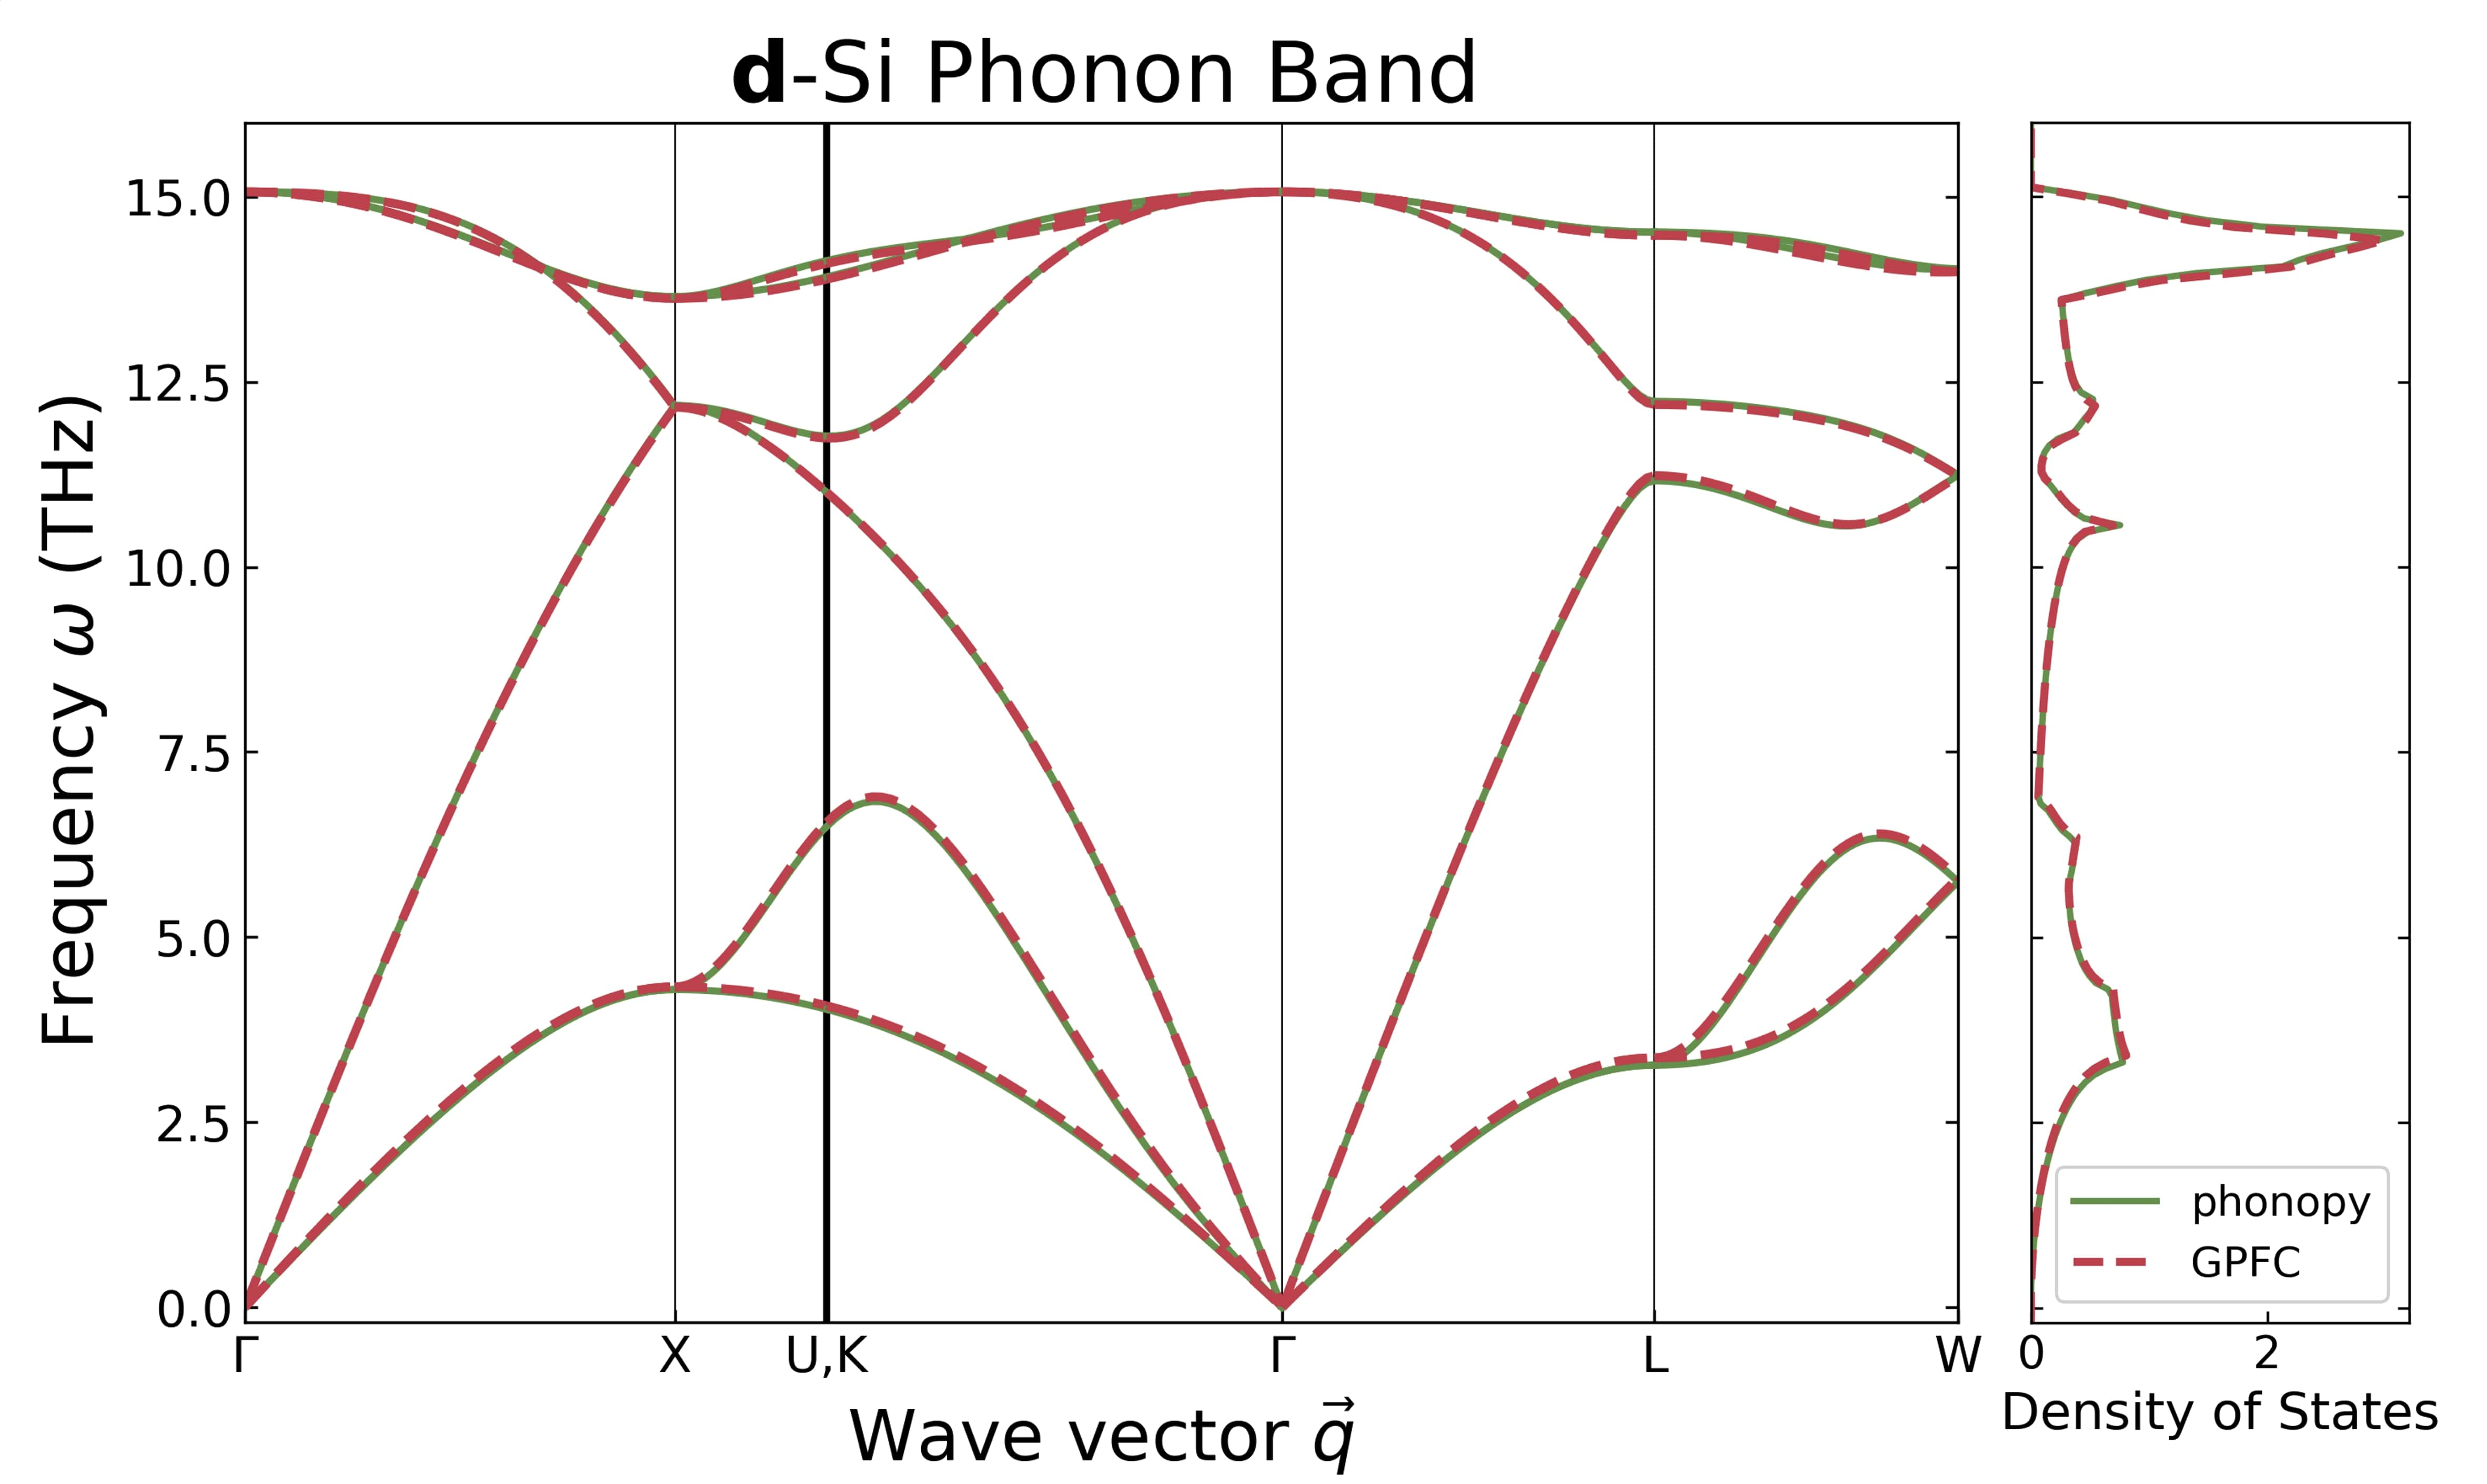
\includegraphics[width=1\linewidth,height=\textheight,keepaspectratio]{Figure/Chapter 3/Cart_results/FC2/d-Si.jpg}
  \caption{}
\end{subfigure}%
\begin{subfigure}{.5\textwidth}
  \centering
  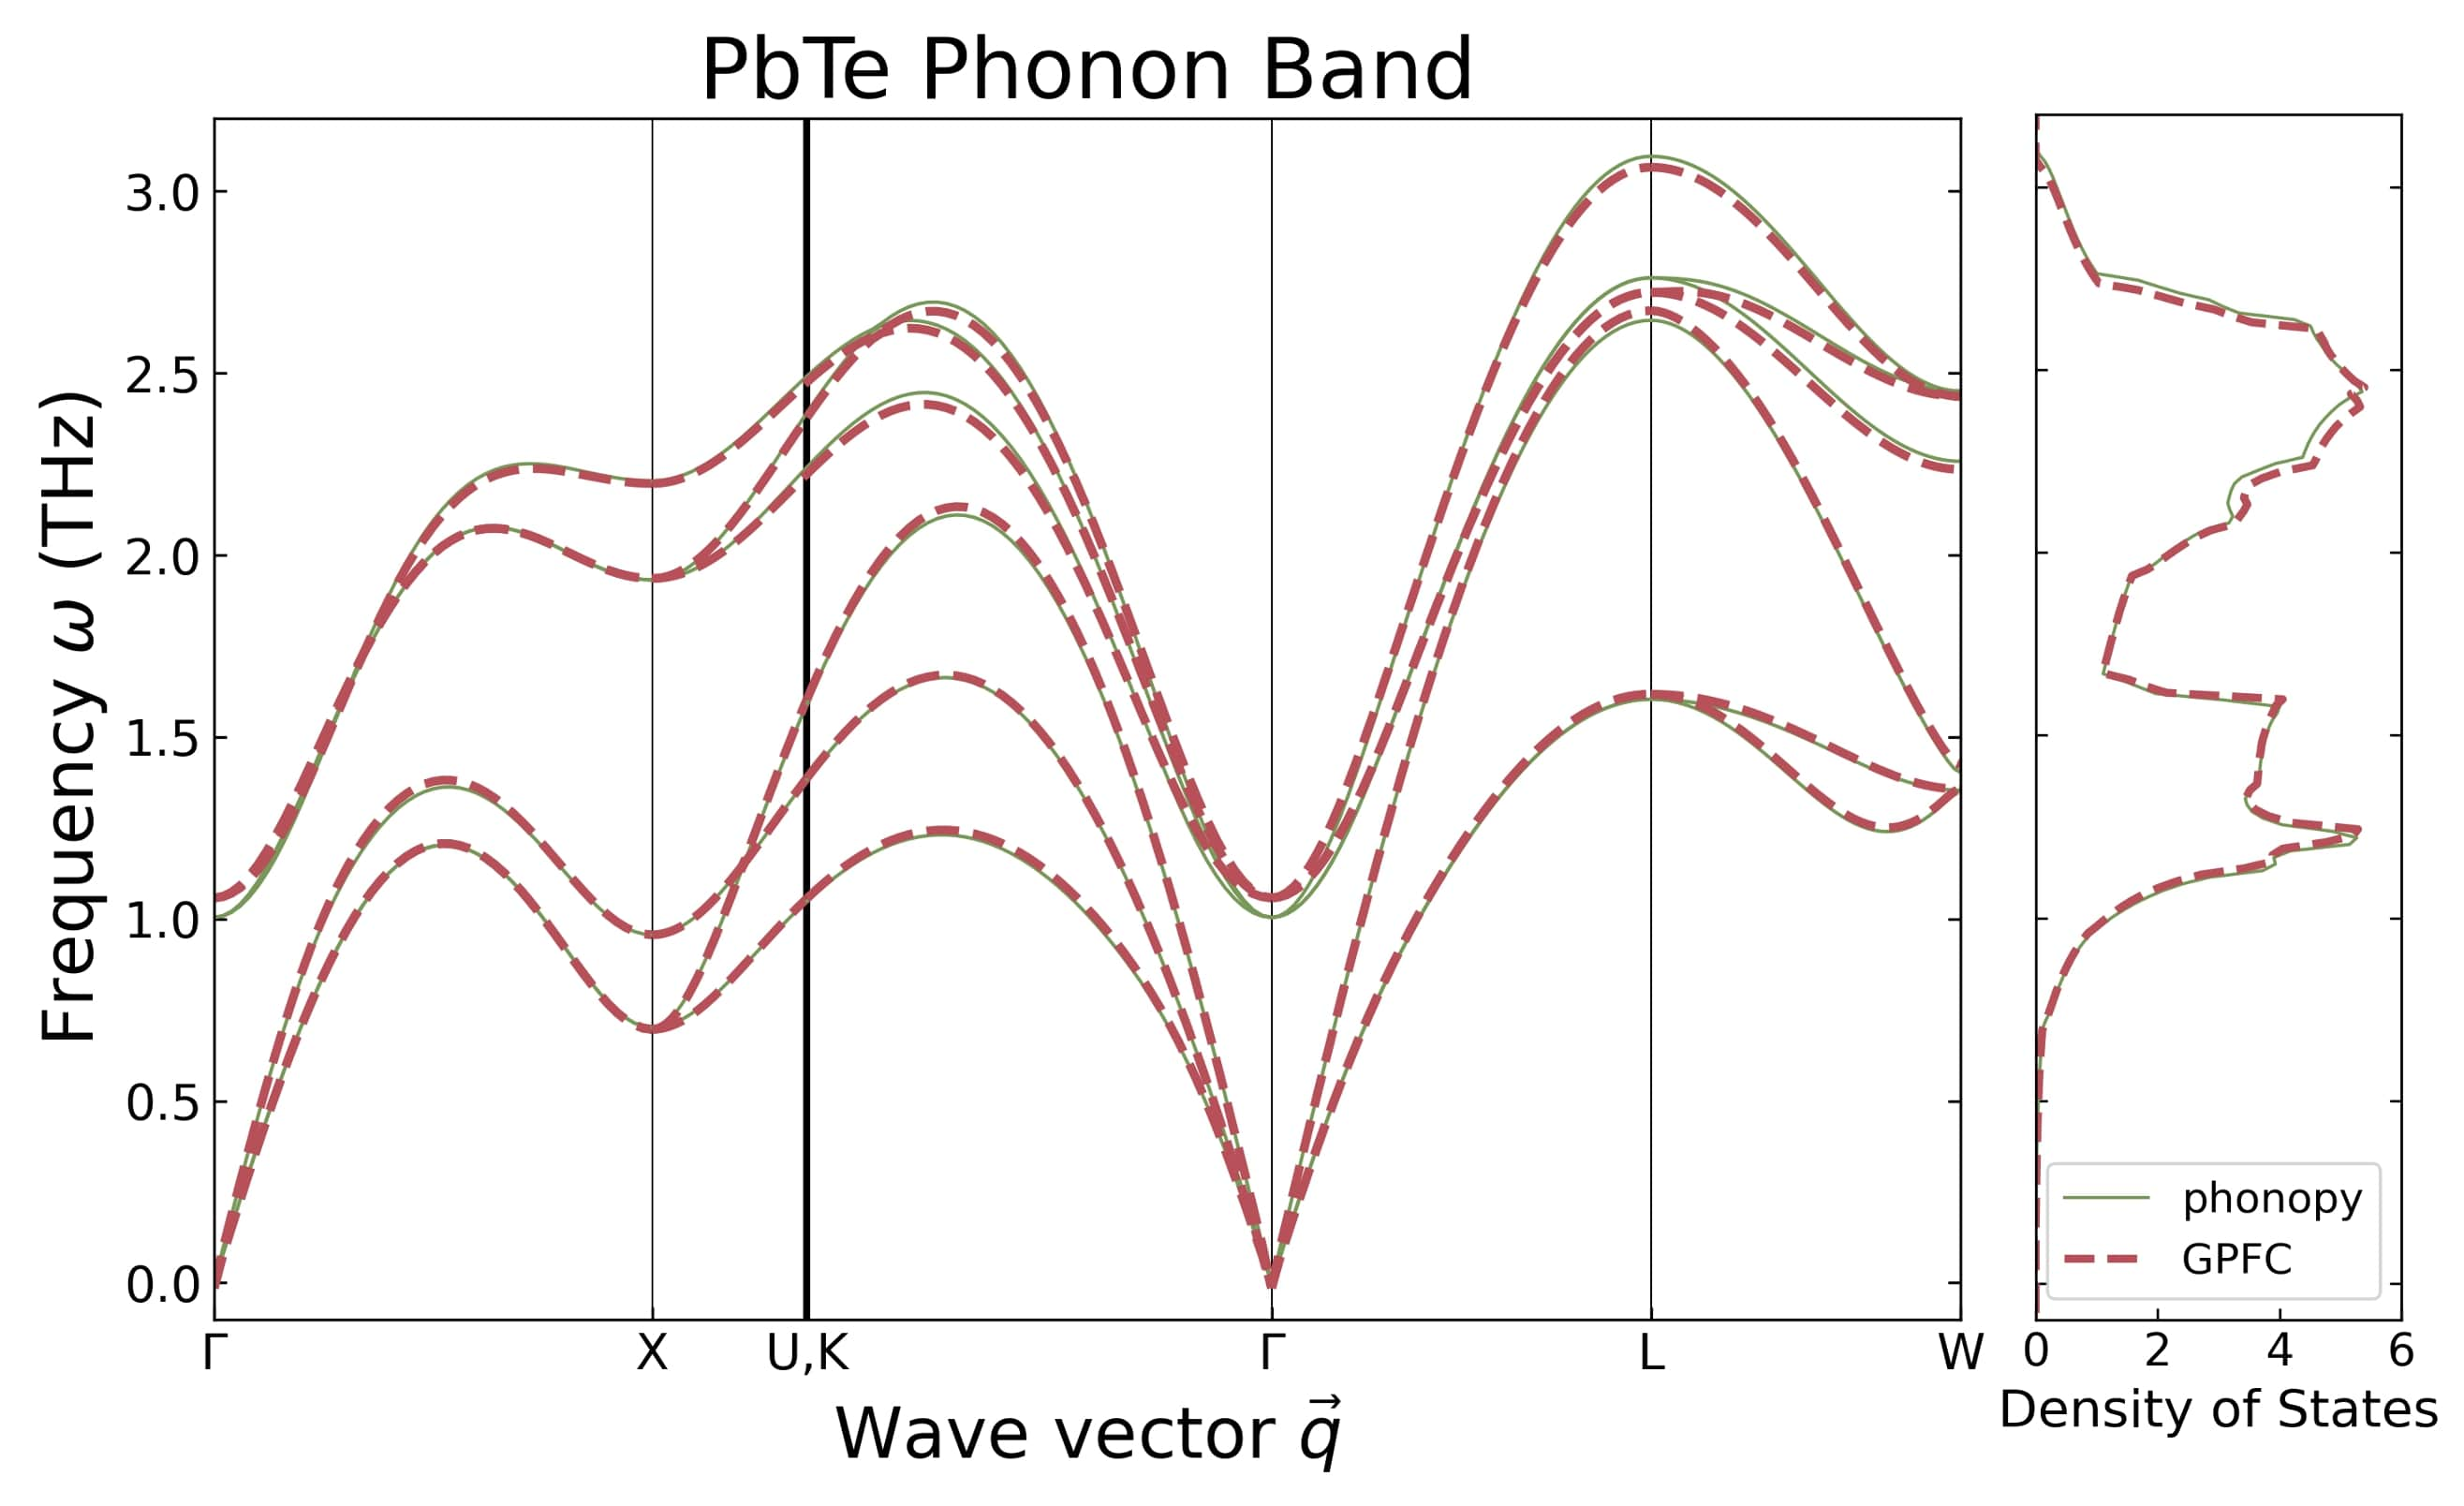
\includegraphics[width=1\linewidth,height=\textheight,keepaspectratio]{Figure/Chapter 3/Cart_results/FC2/PbTe.jpg}
  \caption{}
\end{subfigure}
\caption{
    \label{fig:3.4}
    Panels (a) and (b) show the phonon band structures and density of states for d-\textbf{Si} and \textbf{PbTe}, respectively. 
    %Solid green lines represent results computed using FC2 values from \textsc{Phonopy} (FDM), while dashed red lines correspond to results from our GPFC2 predictions.
}
\end{figure*}

We include supplementary comparisons of phonon band structures and phonon density of states, calculated using our GPFC2, with those computed from the FDM-based FC2s for the remaining materials (\textbf{GaAs}, \textbf{CdTe}, and \textbf{NaCl}) in Appendix~\ref{sec:A.2.1}. Additionally, in Appendix~\ref{sec:A.2.4} we compare our d-\textbf{Si} phonon results with the phonon band structures and phonon density of states evaluated using the FC2 based on the cluster expansion method, \textsc{HiPhive} \cite{Eriksson2019}.

To evaluate the accuracy of cubic anharmonic (third-order) force constants predicted by our model, we present RMSE learning curves analogous to those used for GPFC2 in Figure~\ref{fig:3.3}~(b). Based on the convergence behaviour, accurate prediction of third-order force constants in a Cartesian basis requires approximately 400 energy and force evaluations.

We further assess the physical reliability of these predicted cubic force constants by computing finite-temperature phonon lifetimes and lattice thermal conductivities for five materials: d-\textbf{Si}, \textbf{NaCl}, \textbf{PbTe}, \textbf{GaAs}, and \textbf{CdTe}, over a temperature range of 300–1200~K. These quantities are calculated using third-order many-body perturbation theory as implemented in \textsc{Phono3py}, with input FC3s generated either via finite displacement methods (FDM) or our GP-based approach (GPFC). The cubic anharmonic GP force constants are predicted using Equation~\eqref{equ:3.9}, with the same training data used for the harmonic GPFC2 model.

\begin{figure*}[t]
\centering
\begin{subfigure}{.5\textwidth}
  \centering
  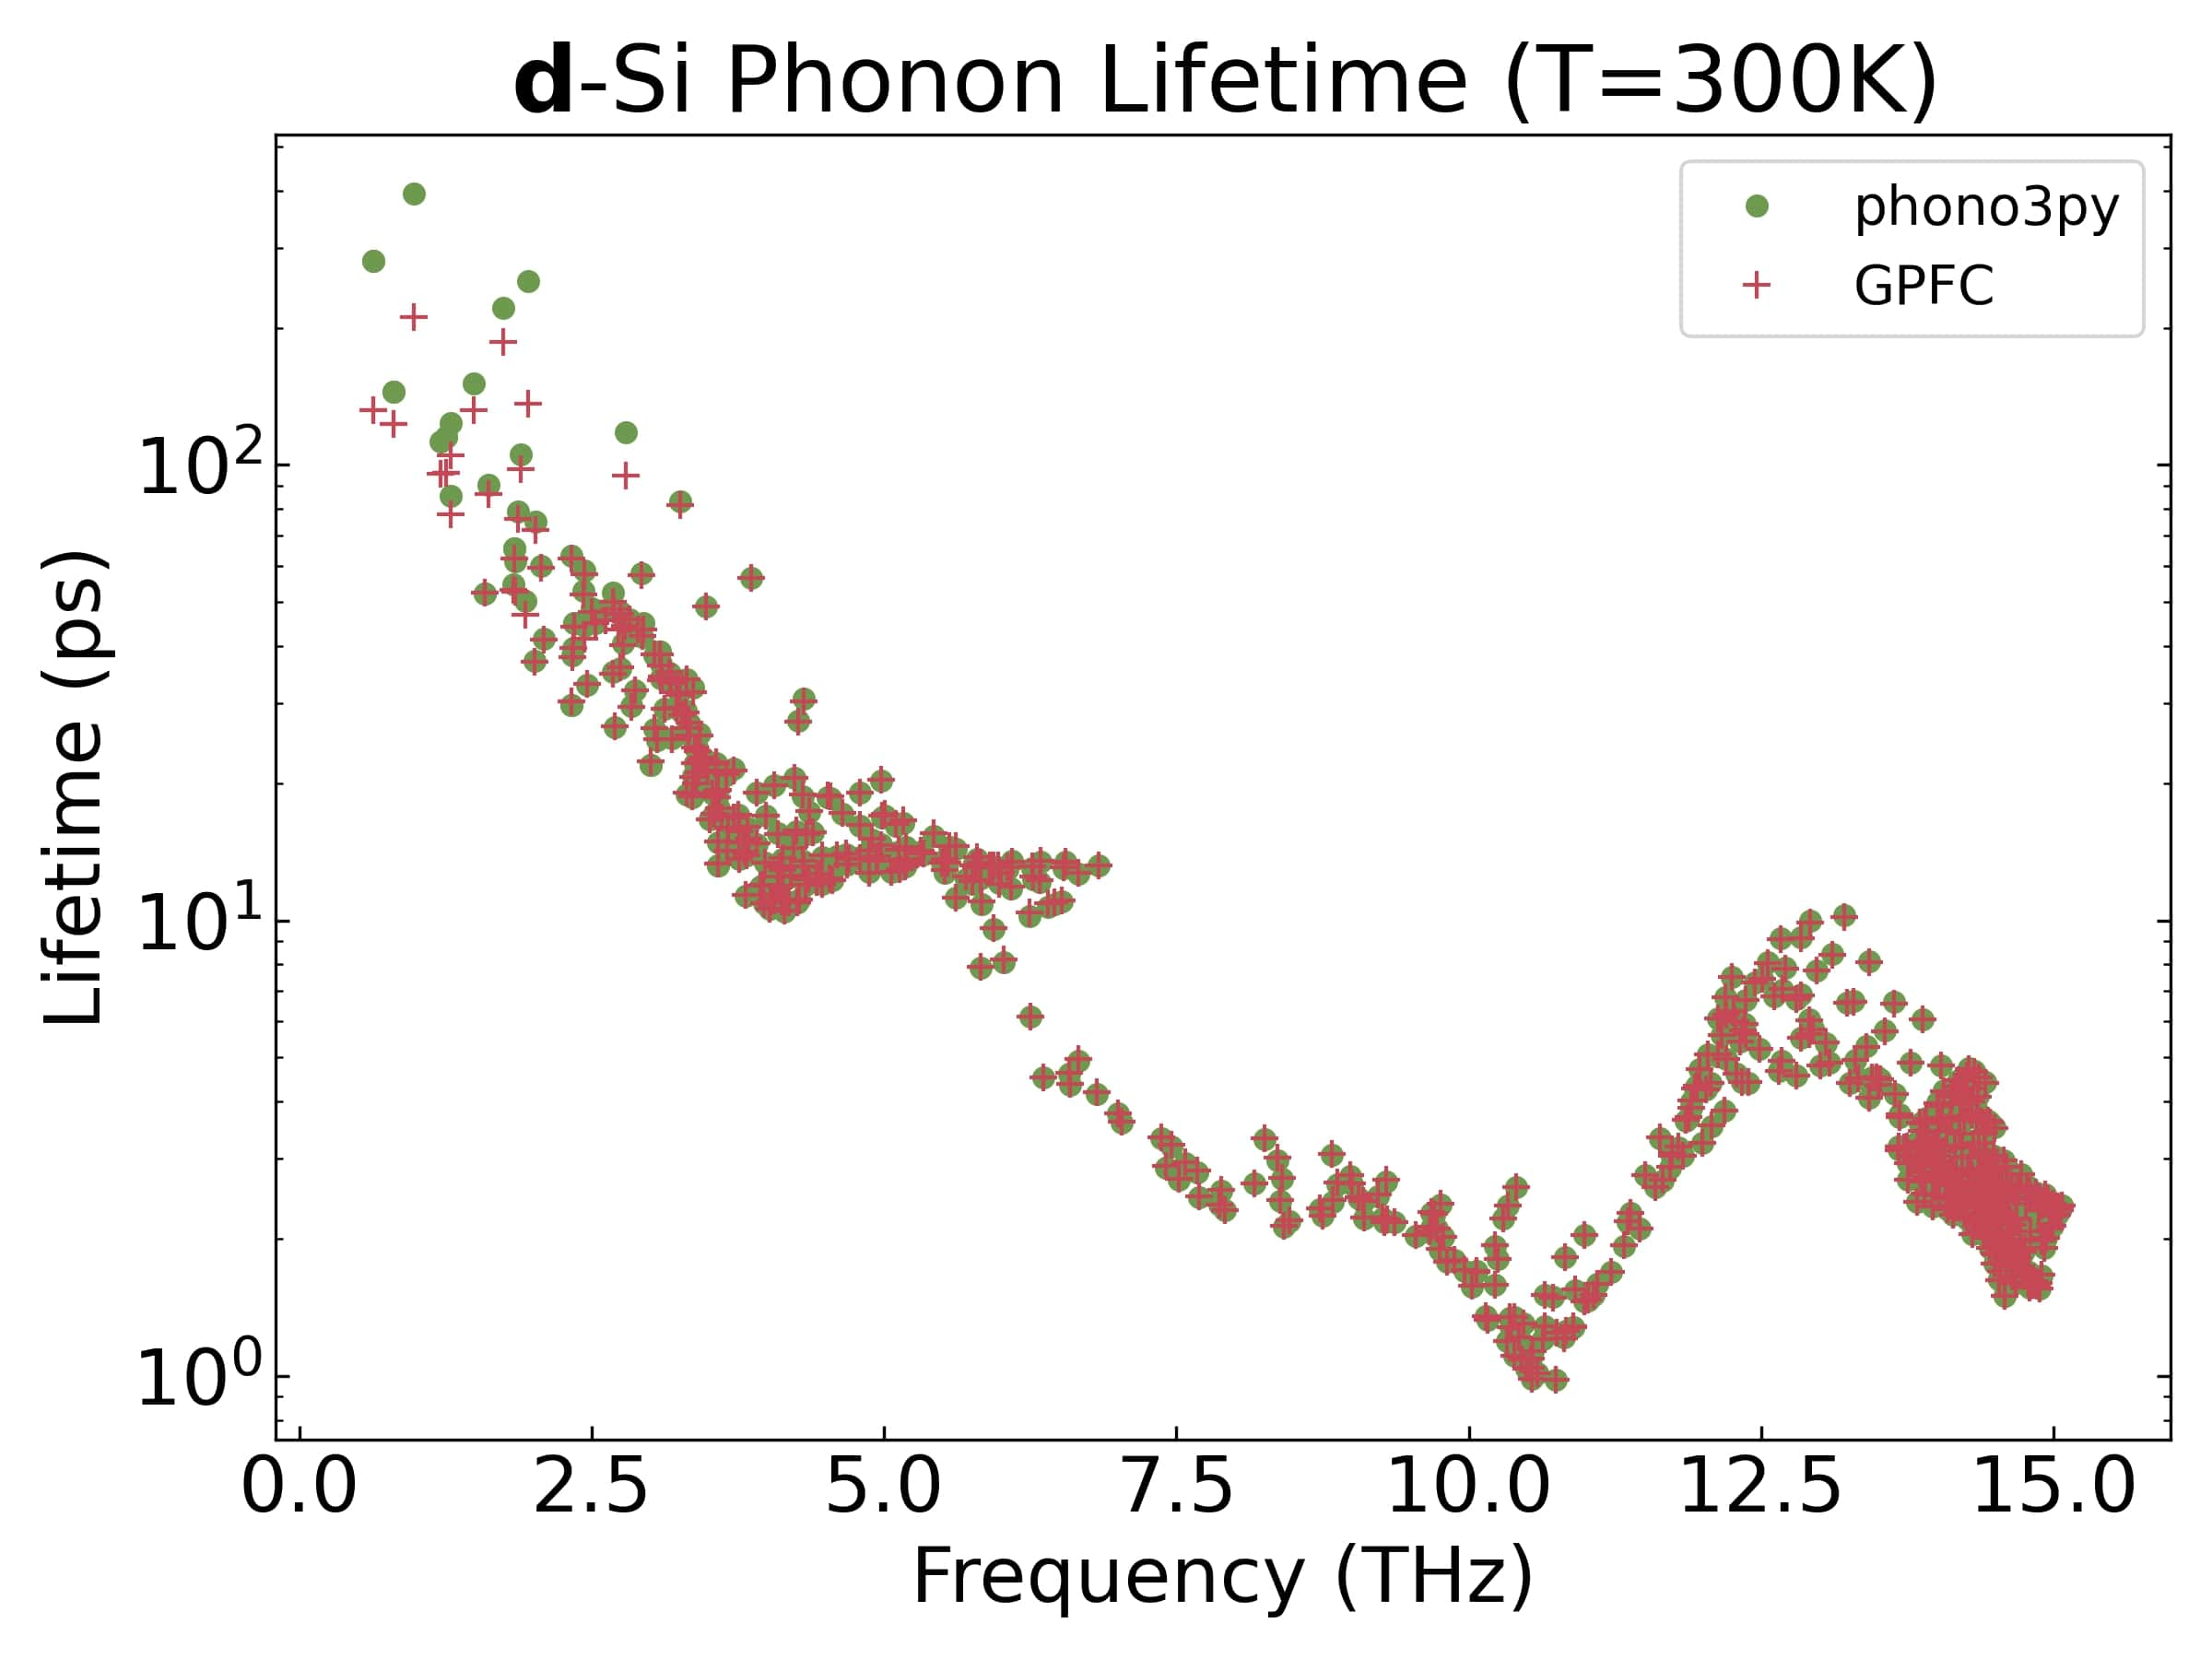
\includegraphics[width=\linewidth,keepaspectratio]{Figure/Chapter 3/Cart_results/FC3/d-Si_pLT_300K.jpg}
  \caption{}
\end{subfigure}%
\begin{subfigure}{.5\textwidth}
  \centering
  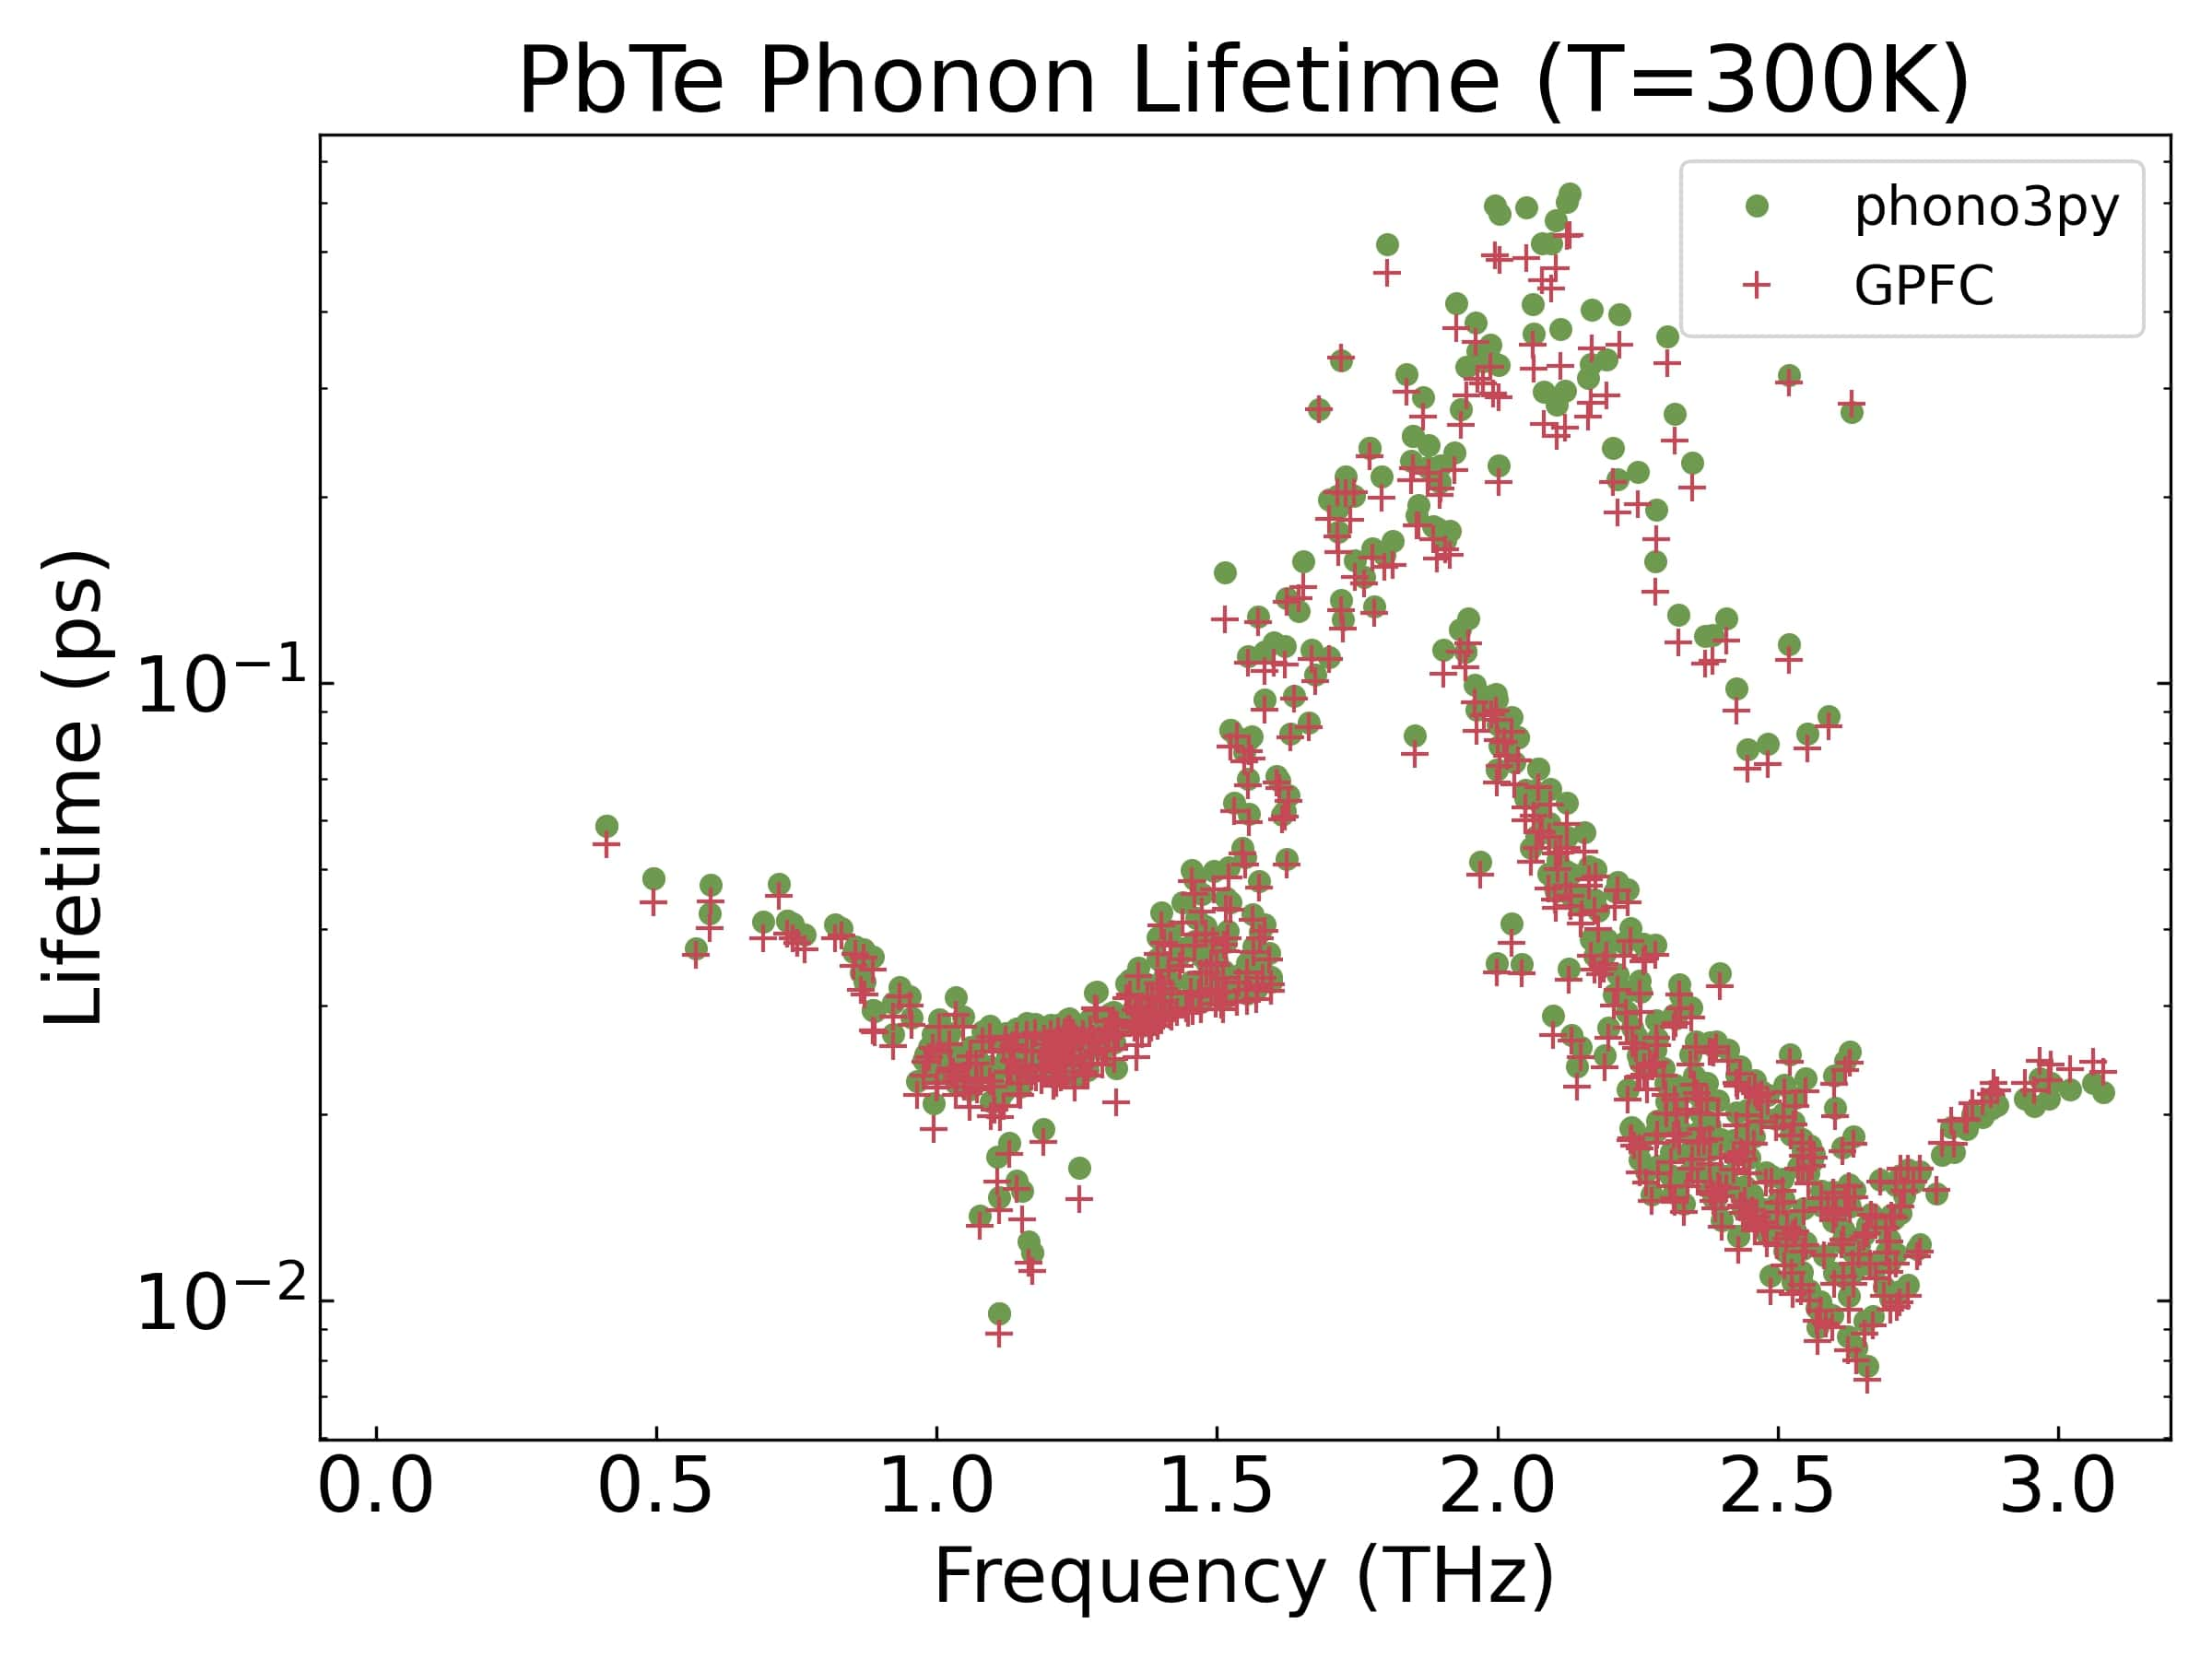
\includegraphics[width=\linewidth,keepaspectratio]{Figure/Chapter 3/Cart_results/FC3/PbTe_pLT_300K.jpg}
  \caption{}
\end{subfigure}

\caption{
    \label{fig:3.5}
    These figures show the predicted phonon lifetimes at 300~K of d-\textbf{Si} and \textbf{PbTe}. %Green point clouds are the result of using cubic anharmonic force constants calculated with \textsc{Phono3py} via FDM, while red point clouds are predicted based on GPFC3.
}
\end{figure*}

\begin{figure*}[t]
\centering
\begin{subfigure}{.5\textwidth}
  \centering
  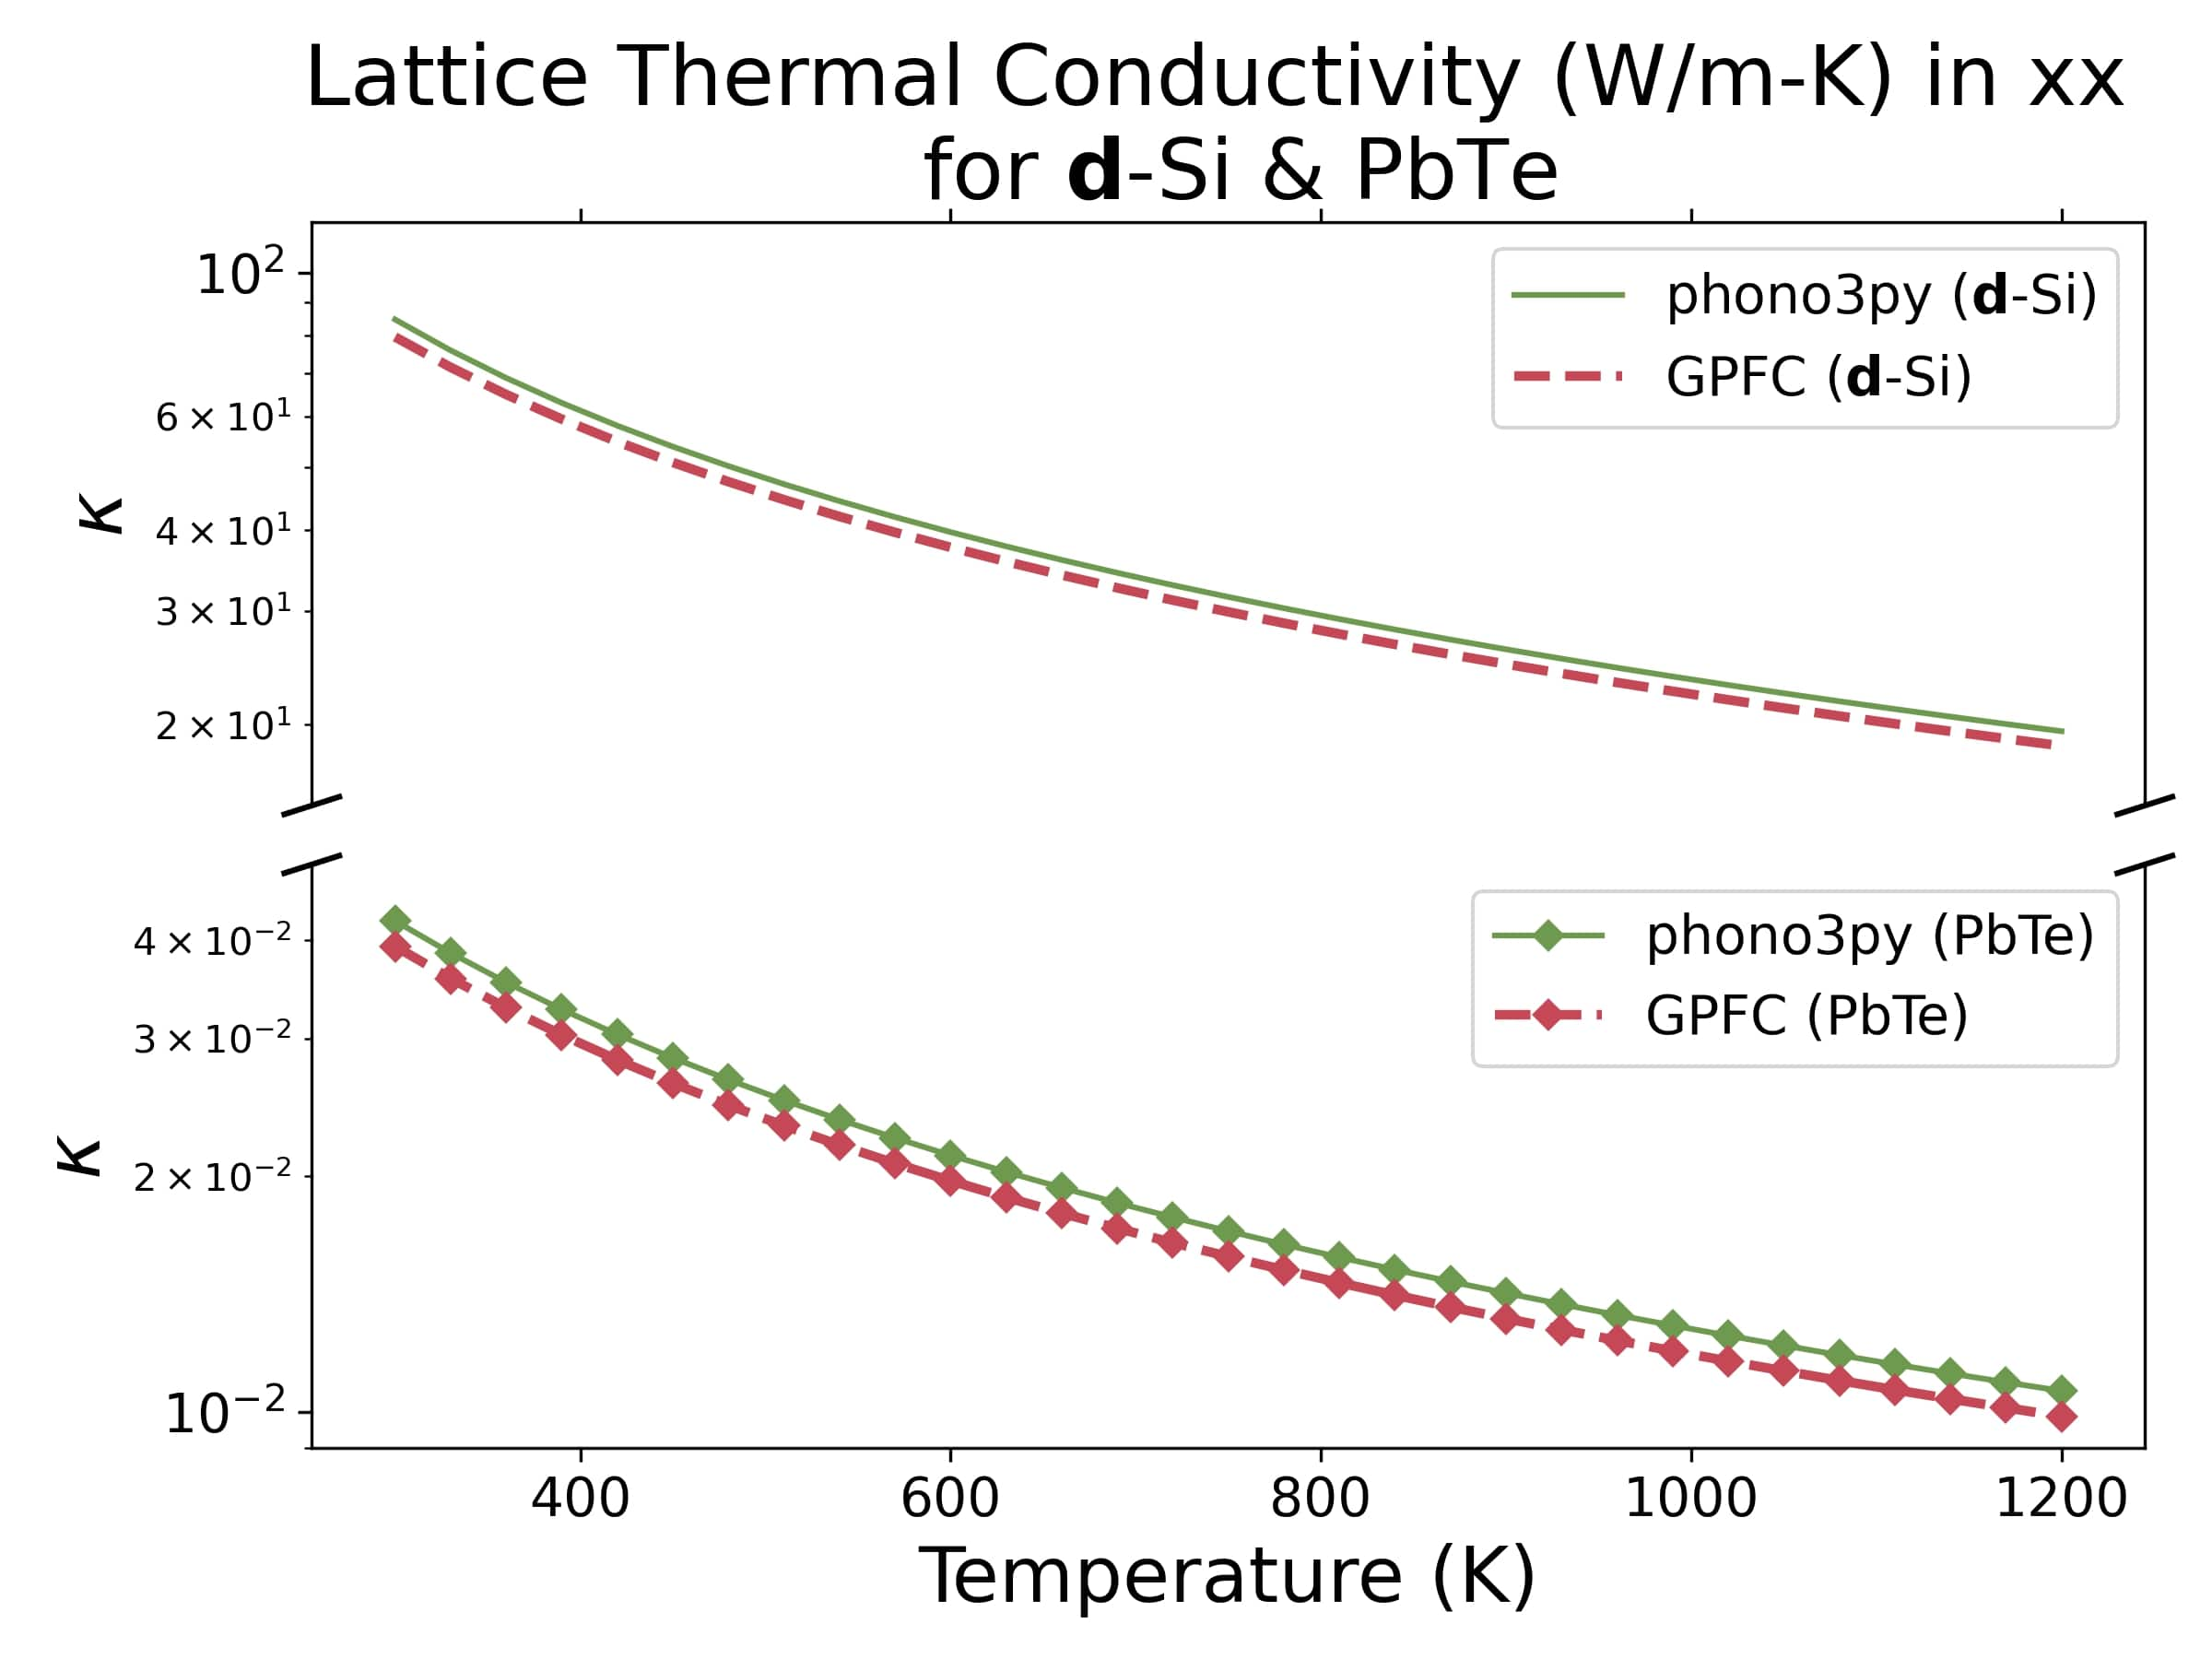
\includegraphics[width=\linewidth,keepaspectratio]{Figure/Chapter 3/Cart_results/FC3/Kappa.jpg} % Replace with your new image
  \caption{}
\end{subfigure}

\caption{
    \label{fig:3.6}
    This figure illustrates the lattice thermal conductivities of d-\textbf{Si} and \textbf{PbTe} over the temperature range from 300~K to 1200~K. %Green and red lines correspond to results obtained using cubic anharmonic force constants calculated with \textsc{Phono3py} via FDM and the predictions based on GPFC3, repectively.
}
\end{figure*}


Figure~\ref{fig:3.5} presents the predicted phonon lifetimes for d-\textbf{Si} and \textbf{PbTe} at 300~K in panels (a) and (b), respectively. The corresponding lattice thermal conductivities are shown in Figure~\ref{fig:3.6}.
To quantify differences in phonon lifetimes across temperatures, we compute the Earth Mover Distance (EMD) between the lifetime density of states at 30~K intervals from 300~K to 1200~K.
The mean EMD values are $3.9 \times 10^{-1}$~ps for d-\textbf{Si} and $8.6 \times 10^{-3}$~ps for \textbf{PbTe}, indicating high fidelity of the GPFC3 predictions, particularly for the latter.

The mean absolute errors in lattice thermal conductivity predictions using GPFC3 are $2.03$~W$\cdot$m$^{-1}$K$^{-1}$ (MAE $\approx$ 2.87\% error) for d-\textbf{Si}, and $1.4 \times 10^{-3}$~W$\cdot$m$^{-1}$K$^{-1}$ (MAE$\approx$ 7.48\% error) for \textbf{PbTe}. Additional results for \textbf{NaCl}, \textbf{GaAs}, and \textbf{CdTe}, also computed with GPFC3, exhibit relative errors in the range of 2–7\%.

Among all studied systems, the lowest accuracy of GPFC3 is observed in \textbf{PbTe}, which is known to exhibit strong anharmonicity and pronounced phonon–phonon interactions that shorten phonon lifetimes and challenge model generalisation.

Supplementary comparisons of phonon lifetimes and lattice thermal conductivities for \textbf{GaAs}, \textbf{CdTe}, and \textbf{NaCl} are also provided in Appendix~\ref{sec:A.2.2}.

It is important to note that the GPFC framework does not offer a computational speed advantage over conventional finite-displacement approaches implemented in \textsc{Phonopy} or \textsc{Phono3py}. 
In all applications presented here, the GPFC calculations are in fact slower, primarily due to the analytical evaluation of higher-order kernel derivatives and the absence of symmetry exploitation, which substantially increases the number of degrees of freedom. 
However, the purpose of GPFC is methodological generality rather than speed. 
Because the present implementation does not impose crystal symmetry, the model can be directly applied to systems with low or broken symmetry—such as amorphous materials, molecular crystals, or interfacial structures—where traditional finite-displacement or symmetry-based lattice-dynamics approaches become inefficient or ambiguous. 
Therefore, although slower for highly symmetric crystals, the GPFC method provides a unified, symmetry-agnostic framework that can extract harmonic and anharmonic force constants consistently from general atomic configurations.

\paragraph{}
While the Cartesian descriptor provides a straightforward and general representation of atomic displacements, it does not exploit the underlying symmetries of the crystal lattice—such as translational invariance and dynamical matrix sparsity—which can lead to redundancy in the model and increased data requirements. To address this, we will introduce a phonon-mode-based descriptor that inherently incorporates lattice symmetries and reduces the dimensionality of the learning problem.
In the following section, we present how this descriptor is implemented in \textsc{GPFC.jl}, analyse its impact on model efficiency and accuracy, and compare its learning behaviour with that of the Cartesian approach.

\newpage
\section{\textsc{GPFC.jl} with Phonon descriptors} \label{sec:3.2}
\paragraph{}
In another section of our previous work~\cite{https://doi.org/10.48550/arxiv.2405.05113}, we investigate a different strategy based on phonon coordinates, or normal modes, as input descriptors for the Gaussian process model rather than straight Cartesian representations.
These normal modes form a natural basis for atomic motion in a crystalline material or molecule and inherently encode the symmetries of the system.
Moreover, they serve as the foundation for higher-order theoretical frameworks in lattice dynamics, such as many-body perturbation theory, which couples normal modes through anharmonic interactions.

\subsection{Phonon descriptors} \label{subsec:3.2.1}
Our motivation for using phonon-mode descriptors is to improve the efficiency of the machine learning model—achieving higher accuracy with fewer training data—without explicitly encoding symmetry or equivariance in the model architecture. The normal modes are obtained by diagonalising the mass-weighted second-order force constant matrix, also known as the dynamical matrix.

Before constructing phonon descriptors, we now revisit the expression of the ``\textit{Dynamical Matrix}'' \cite{phonopy, Togo2015-qf, Phonopy_toolkit} at wave vector $\textbf{q}$:
\begin{equation}
\label{equ:3.17}
    \begin{split}
        D_{\alpha\beta,\;\kappa\kappa'}(\mathbf{q}) =  \frac{1}{\sqrt{m_{(\kappa)}m_{(\kappa')}}}\sum_{l'}\Phi^{(2)}_{\alpha l\kappa,\;\beta l'\kappa'}\:\textbf{e}^{i\mathbf{q}\cdot\left(\mathbf{R}^{0}_{\kappa' l'}-\mathbf{R}^{0}_{\kappa l}\right)},
    \end{split}
\end{equation} 
%
where the masses \( m_{(\kappa)} \) and \( m_{(\kappa')} \) correspond to atoms \( \kappa \) and \( \kappa' \) in unit cells \( l \) and \( l' \), respectively.  
The term \( \Phi^{(2)}_{\alpha l\kappa,\;\beta l'\kappa'} \) is the harmonic force constant between components \( \alpha \) and \( \beta \) of atoms \( \kappa \) and \( \kappa' \) in cells \( l \) and \( l' \).  
The vectors \( \mathbf{R}^{0}_{\kappa l} \) and \( \mathbf{R}^{0}_{\kappa' l'} \) denote their respective equilibrium positions.  
The summation runs over all primitive cells \( l' \), with \( l = 0 \) referring to the reference cell.

Equation~\eqref{equ:3.17} can be interpreted as the discrete Fourier transform of the harmonic force constants expressed in the Cartesian basis.
By analogy, we can apply a similar transformation to the atomic displacement descriptors themselves.
Specifically, we recast the Cartesian descriptors in reciprocal space and obtain the phonon-mode descriptor as
\begin{tcolorbox}[
    ams equation,
    title=Phonon descriptor,
    %colback=blue!5,
    colframe=bEpic,
    %colframe=blue!75!black,
    coltitle=white,
    %fontupper=\color{blue}  % << changes font color inside the box
]
 \label{equ:3.18}
\begin{split}
    d_{\beta\kappa'}(\mathbf{q}) = 
    \sqrt{m_{\kappa'}} 
    \sum_{l'} \mathbf{x}_{\beta l' \kappa'} \,
    e^{i \mathbf{q} \cdot \left( \mathbf{R}^{0}_{\kappa' l'} - \mathbf{R}^{0}_{\kappa l} \right)},
\end{split}
\end{tcolorbox}

where \( \mathbf{x}_{\beta l'\kappa'} \) are the atomic displacement descriptors in Cartesian coordinates, \( m_{\kappa'} \) is the mass of atom \( \kappa' \), and \( \mathbf{R}^{0}_{\kappa' l'} \) denotes the equilibrium position of the atom \( \kappa' \) in the unit cell \( l' \). The resulting quantity \( d_{\beta\kappa'}(\mathbf{q}) \) represents the projection of atomic displacements onto the vibrational normal modes at wavevector \( \mathbf{q} \), and is analogous to the phonon eigenvector components obtained from diagonalising the dynamical matrix.

\begin{figure*}[t]
\centering
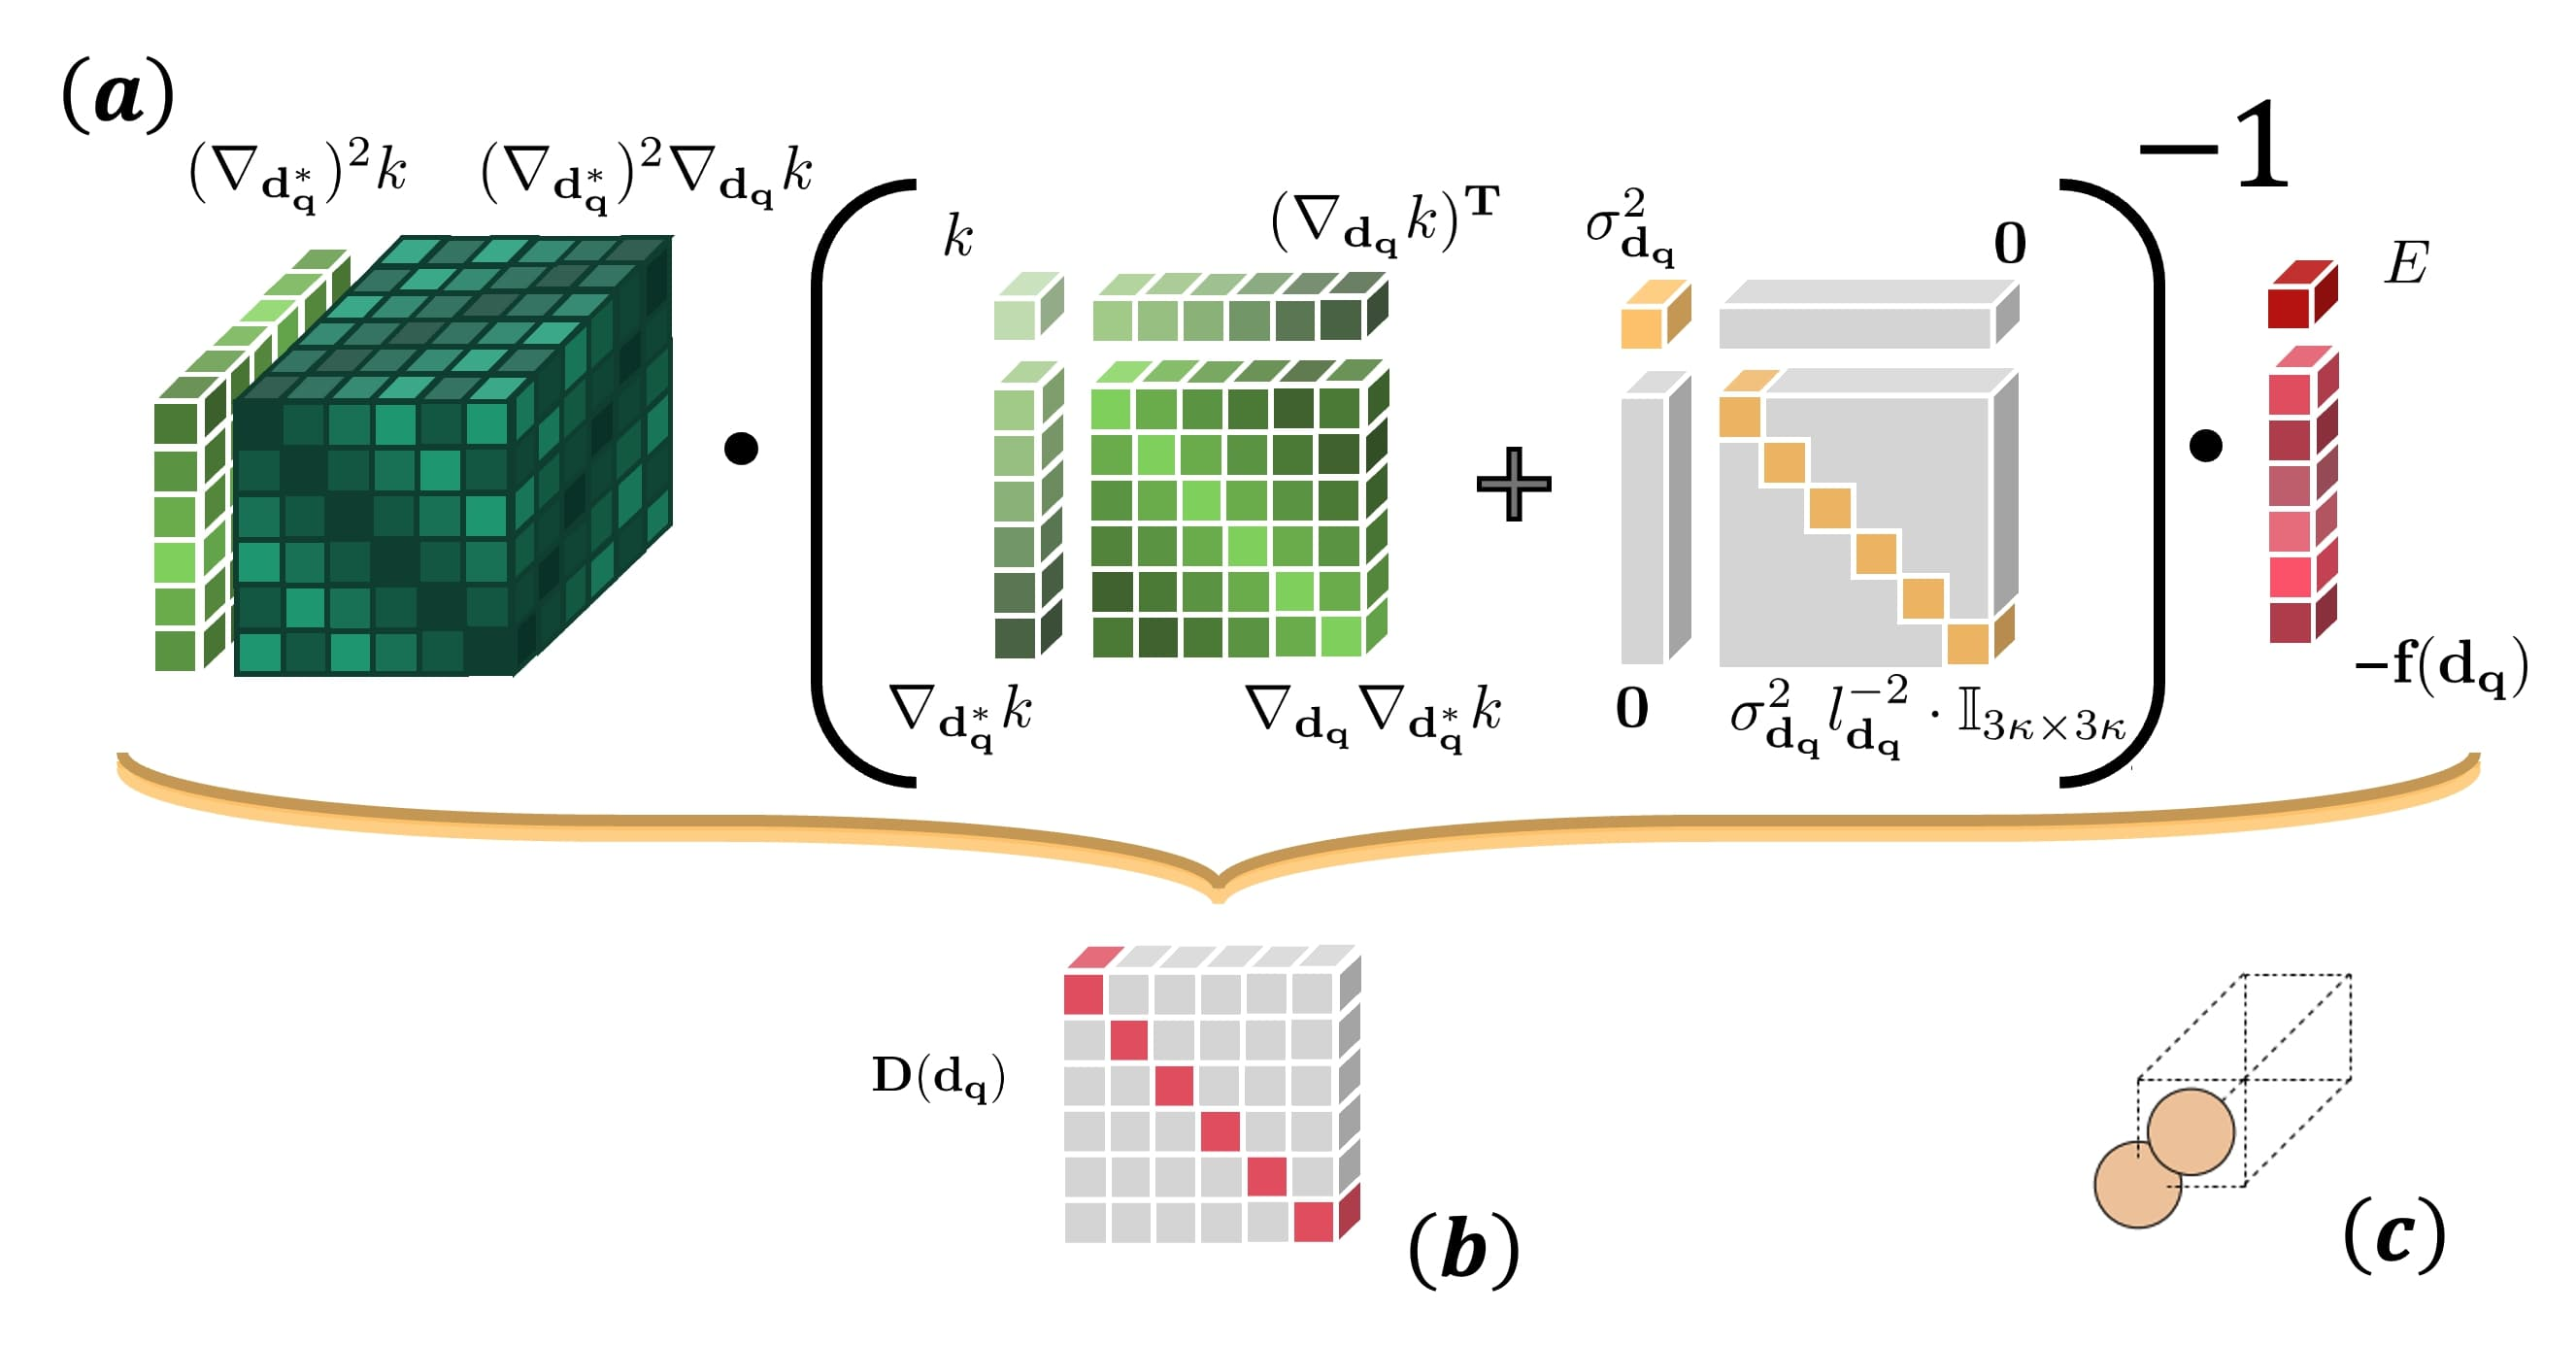
\includegraphics[width=1.0\textwidth]{Figure/Chapter 3/GPFC_phono.jpg}
\caption{\label{fig:3.7} \label{fig:2} 
Figure illustrates the tensor contraction in Equation~\eqref{equ:3.7} using phonon-mode descriptors. %The resulting quantity in panel (3.8b) is the dynamical matrix \( \mathbf{D}(\mathbf{d}_{\mathbf{q}}) \), rather than the harmonic force constant tensor, corresponding to the analysis of a primitive silicon crystal, as shown in panel (3.8c). \cite{https://doi.org/10.48550/arxiv.2405.05113}.
}
\end{figure*}

Integrating the phonon descriptor directly imposes the system's symmetry in our GP model, which removes the requirement for the model to infer these symmetries from data.  
Moreover, the descriptor dimensionality is significantly decreased: the model performs on a primitive cell that includes just $\kappa$ atoms, unlike a complete $l \times l \times l$ supercell. 
This means that while there are $N = l^{3} \kappa$ atoms in the atomic environment, the phonon-based descriptors reduce this information to the size of the primitive cell.
As seen in Figure~\ref{fig:3.7}, the equivalent tensor contraction, which was first represented in Equation~\eqref{equ:3.7}, can be redefined appropriately as
\begin{tcolorbox}[
    ams equation,
    title=Phonon-basis GPFC2 prediction,
    %colback=blue!5,
    colframe=bEpic,
    %colframe=blue!75!black,
    coltitle=white,
    %fontupper=\color{blue}  % << changes font color inside the box
]
\label{equ:3.19}
\begin{split}
    \mathbf{D}(\mathbf{d}^{*}_{\mathbf{q}}) = 
    \begin{bmatrix}
          (\nabla_{\mathbf{d}^{*}_{\mathbf{q}}})^2 k &
          (\nabla_{\mathbf{d}^{*}_{\mathbf{q}}})^2 \nabla_{\mathbf{d}_{\mathbf{q}}} k
    \end{bmatrix}_{\mathbf{d}_{\mathbf{q}},\;\mathbf{d}^{*}_{\mathbf{q}}}
        \cdot \mathcal{K}^{-1}_{\mathbf{d}_{\mathbf{q}},\: \mathbf{d}_{\mathbf{q}}}
        \cdot
        \begin{bmatrix}
              E \\
              -\mathbf{f}
        \end{bmatrix}_{\mathbf{d}_{\mathbf{q}}},
\end{split}
\end{tcolorbox}
where $\mathbf{D}(\mathbf{d}^{*}_{\mathbf{q}})$ denotes the dynamical matrix evaluated at wavevector $\mathbf{q}$ and $\mathbf{f}$ is the phonon-basis force obeyed the discrete Fourier transform in \eqref{equ:3.18}.
The prediction of GPFC3 can be recast in a form analogous to the GPFC2 expression derived above.


For a training set of size \( m \), the computational cost of learning—dominated by the inversion of a \( (m \cdot (1 + 3N)) \times (m \cdot (1 + 3N)) \) covariance matrix—is \( \mathcal{O}(m^{3} \cdot (1 + 3N)^{3}) \). Similarly, the cost of prediction—arising from the dot product of two vectors of dimension \( m \cdot (1 + 3N) \)—is \( \mathcal{O}(m \cdot (1 + 3N)) \)~\cite{RasmussenW06, David}. By employing phonon-mode descriptors, where the input dimensionality is reduced from the full atomic environment (\( N \) atoms) to that of the primitive cell (\( \kappa \) atoms), these costs are reduced to \( \mathcal{O}(m^{3} \cdot (1 + 3\kappa)^{3}) \) for training and \( \mathcal{O}(m \cdot (1 + 3\kappa)) \) for prediction, respectively.

\subsection{Phonon-basis GPFC} \label{subsec:3.2.2}
We also compare our phonon-based GPFC2 and GPFC3 predictions with the dynamical matrix and third-order force constants (FC3) obtained from the finite displacement method (FDM), as implemented in \textsc{Phono(3)py}. The same dataset used for the Cartesian-basis models in Section~\ref{subsec:3.2.2}—comprising five representative materials (d-\textbf{Si} (FCC), \textbf{GaAs}, \textbf{CdTe}, \textbf{NaCl}, and \textbf{PbTe})—is employed to train the derivative GP model using phonon-mode descriptors, enabling the prediction of Gaussian process force constants in the phonon basis.

All GPFC predictions are evaluated at the $\Gamma$-point, as the current implementation of automatic differentiation limits predictions at arbitrary \textbf{q}-points.
We will discuss the extended procedure to address this limitation in the next subsection.
\begin{figure*}[t]\centering
\begin{subfigure}{.5\textwidth}
  \centering
  \includegraphics[width=1\linewidth,height=\textheight,keepaspectratio]{Figure/Chapter 3/Phonon_results/gpfc2_ph.jpg}
  \caption{}
\end{subfigure}%
\begin{subfigure}{.5\textwidth}
  \centering
  \includegraphics[width=1\linewidth,height=\textheight,keepaspectratio]{Figure/Chapter 3/Phonon_results/gpfc3_ph.jpg}
  \caption{}
\end{subfigure}
    \caption{
        \label{fig:3.8}
        Learning curves in (a) and (b) illustrate the direct comparison of GPFC2 and GPFC3 in phonon descriptors to FC2 and FC3 from FDM, respectively, using \textsc{Phono(3)py}. %Yellow, green, blue, pink and red colours represent d-\textbf{Si} (FCC), \textbf{GaAs}, \textbf{CdTe}, \textbf{NaCl} and \textbf{PbTe}. The dashed-dot lines denote the force constant in the phonon basis (predicted at gamma: $\Gamma$ point).
    }
\end{figure*}
The accuracy of the GPFC2 and GPFC3 models is shown in Figures~\ref{fig:3.8}(a) and (b), respectively, in terms of root mean square error (RMSE) learning curves. The RMSE of GPFC2 predictions converges rapidly to near-zero values using only $6$–$10$ training points, while the GPFC3 model requires approximately $30$–$50$ data points to achieve comparable accuracy. Compared to the Cartesian-basis results in Figure~\ref{fig:3.3}, these learning curves again reflect the dimensionality of the descriptor: the number of required training samples closely matches the number of degrees of freedom in the phonon descriptor, which corresponds to the number of atoms in the primitive cell.

Moreover, the phonon-based GPFC2 and GPFC3 models also exhibit learning of translational symmetry, as illustrated in Fig.~\ref{fig:A.7}b. The convergence of the acoustic sum rule becomes evident in the learning curves after approximately 10 and 30–50 data points, respectively.

We also observe that predicting the cubic anharmonic force constants (GPFC3) generally requires roughly eight times more training data than is needed to achieve similar accuracy for the harmonic case (GPFC2). 

\subsection{Recovering Real Space FCs} \label{subsec:3.2.3}

Recovering phonon-based force constants into the Cartesian basis is essential for calculating full phonon dispersion relations and lattice thermal conductivity. However, a limitation arises due to current automatic differentiation frameworks, which do not support taking derivatives with respect to complex-valued phonon descriptors beyond second order. As a result, both the harmonic and cubic anharmonic dynamical matrices can only be evaluated at the $\Gamma$-point, where the phonon descriptors are real-valued.

To address this limitation, we propose the construction and implementation of a differentiable Gaussian process model capable of handling complex-valued descriptors. A discussion of this extension, along with the derivation of the relevant complex derivatives, is provided in Appendix~\ref{sec:A.1.2}.

Once the harmonic (GPFC2) and cubic anharmonic (GPFC3) Gaussian process force constants have been computed in the phonon basis, we follow a well-defined procedure to transform them back into the Cartesian basis \cite{phonopy, Togo2015-qf, Phonopy_toolkit}. For the harmonic case, the inverse discrete Fourier transform of the set of dynamical matrices over all $N_{\mathbf{q}}$ wavevectors can be used to recover the real-space force constants as:

\begin{equation}
\label{equ:3.20}
    \Phi^{(2)}_{\alpha l \kappa,\;\beta l' \kappa'} = 
    \frac{ \sqrt{m_{\kappa} m_{\kappa'}} }{N_{\mathbf{q}}}
    \sum_{\mathbf{q}} 
    D_{\alpha \beta,\; \kappa \kappa'}(\mathbf{q}) \,
    e^{-i \mathbf{q} \cdot \left( \mathbf{R}^{0}_{\kappa' l'} - \mathbf{R}^{0}_{\kappa l} \right)}.
\end{equation}

Here, \( N_{\mathbf{q}} = N_x \times N_y \times N_z \) corresponds to the number of \textbf{q}-points sampled from a Monkhorst–Pack grid covering the Brillouin zone. For a \( 2 \times 2 \times 2 \) supercell, we require only 8 \textbf{q}-points.

Similarly, GPFC3 values in the phonon basis can be transformed back to Cartesian coordinates using an expression analogous to the inverse Fourier transform of Equation~\eqref{equ:2.19}:

\begin{equation}
\label{equ:3.21}
\begin{split}
\Phi^{(3)}_{\alpha l_1 \kappa_1,\; \beta l_2 \kappa_2,\; \gamma l_3 \kappa_3}
= \frac{ \sqrt{ m_{\kappa_1} m_{\kappa_2} m_{\kappa_3} } }{ N_{\mathbf{q}}^2 }
\sum_{\mathbf{q}_2, \mathbf{q}_3}
&\Phi^{(3)}_{\alpha \kappa_1,\; \beta \kappa_2,\; \gamma \kappa_3}(\mathbf{q}_2, \mathbf{q}_3) \\
&\times e^{-i \mathbf{q}_2 \cdot \left( \mathbf{R}^{0}_{\kappa_2 l_2} - \mathbf{R}^{0}_{\kappa_1 l_1} \right)} \\
&\times e^{-i \mathbf{q}_3 \cdot \left( \mathbf{R}^{0}_{\kappa_3 l_3} - \mathbf{R}^{0}_{\kappa_1 l_1} \right)} \\
&\times \delta^{*}\left( \mathbf{q}_1 + \mathbf{q}_2 + \mathbf{q}_3 \right),
\end{split}
\end{equation}

where \( \delta^{*}(\mathbf{q}_1 + \mathbf{q}_2 + \mathbf{q}_3) \) enforces momentum conservation and is defined as


\begin{equation}
\label{equ:3.22}
\delta^{*}(\mathbf{q}_1 + \mathbf{q}_2 + \mathbf{q}_3) =
\begin{cases} 
1, & \text{if } \mathbf{q}_1 + \mathbf{q}_2 + \mathbf{q}_3 \text{ is a reciprocal lattice vector}, \\
0, & \text{otherwise}.
\end{cases}
\end{equation}

Note that predicting \( \Phi^{(3)}(\mathbf{q}_2, \mathbf{q}_3) \) using our current GP model is limited to specific \textbf{q}-points. Nevertheless, the GPFC3 predicted at wavevectors \( (\mathbf{q}_2, \mathbf{q}_3) \) corresponds to the cubic anharmonic dynamical matrix in reciprocal space. This quantity is the Fourier transform of the real-space third-order force constants, and represents the linear response of the force on atom \( \kappa_1 \) to displacements with wavevectors \( \mathbf{q}_2 \) and \( \mathbf{q}_3 \).

The relationship between this response and the force in reciprocal space is given by:
\begin{equation}
\label{equ:3.23}
\begin{split}
    F_{\alpha \kappa_1}(\mathbf{q}_1) = &-\frac{1}{\sqrt{l^{3}}} 
\sum_{\beta \kappa_2} \sum_{\gamma \kappa_3}
\Phi^{(3)}_{\alpha \kappa_1,\; \beta \kappa_2,\; \gamma \kappa_3}(\mathbf{q}_2, \mathbf{q}_3)\\
&d_{\beta \kappa_2}(\mathbf{q}_2) \;
d_{\gamma \kappa_3}(\mathbf{q}_3) \;
\delta^{*}(\mathbf{q}_1 + \mathbf{q}_2 + \mathbf{q}_3),
\end{split}
\end{equation}
allowing us to obtain the phonon descriptors \( d_{\alpha \kappa_1}(\mathbf{q}_1) \) from Equation~\eqref{equ:3.18} and use the corresponding force \( F_{\alpha \kappa_1}(\mathbf{q}_1) \) as training data for GPFC3.

For a \( 2 \times 2 \times 2 \) supercell lattice, recovering the full GPFC3 tensor in the Cartesian basis requires evaluating \( N_{\mathbf{q}}^2 = 64 \) cubic anharmonic dynamical matrices, assuming both \( \mathbf{q}_2 \) and \( \mathbf{q}_3 \) are sampled from the same mesh.


\section{Atomic Cluster Expansion Model} \label{sec:3.3}

In this section, we discuss possible approaches to further improve the efficiency of our differentiable Gaussian process (GP) model. Incorporating physical symmetries of atomic structures has proven to be a sensible and effective strategy in several machine learning potentials~\cite{Langer2022}.

As reviewed in Chapters~\ref{sec:2.4} and~\ref{sec:2.5}, Atomic Cluster Expansion (ACE) descriptors offer one of the most efficient local basis sets for representing individual atoms within atomic structures prior to training the GP model. This is because they are systematically constructed to capture the atomic environment while inherently satisfying permutation, translation, reflection, and rotation symmetries, as shown in Equations~\eqref{equ:2.68},~\eqref{equ:2.69}, and~\eqref{equ:2.76}.

To integrate ACE descriptors with our model, we employ a \textsc{Julia}-language implementation of the ACE framework, the \textsc{ACEpotentials.jl} package~\cite{Witt2023}. \textsc{ACEpotentials.jl} builds upon the foundational concepts of ACE~\cite{Drautz2019, Dusson2022}, incorporating several extensions such as smoothness priors, robust parameter estimation, and an extended design space for capturing atomic species through radial basis functions.
These features make \textsc{ACEpotentials.jl} a simple, interpretable, and robust framework, well-suited for use in our differentiable GP model.

\subsection{ACE descriptors} \label{subsec:3.3.1}

This section aims to investigate the construction of ACE descriptors using the \textsc{ACEpotentials.jl} package and to assess their compatibility and efficiency when incorporated into our differentiable GP model. 

In an $N$-atom structure, ACE descriptors which represent the centred atom $i$ as a \textbf{symmetrised many-body product basis} set $\mathbf{B}_{i}$.
This basis set can be written as the set consisting of the many-body product basis from $1$-body order to $(\nu+1)$-body order expressed as 
\begin{equation} \label{equ:3.24}
    \mathbf{B}_{i} = 
    \begin{bmatrix}
        \mathbf{B}^{(0)}_{i} &
        \mathbf{B}^{(1)}_{i} &
        \mathbf{B}^{(2)}_{i} &
        &\cdots&
        \mathbf{B}^{(\nu)}_{i}
    \end{bmatrix}^{\text{T}},
\end{equation}
where $\mathbf{B}^{(\nu)}_{i}$ are defined in \eqref{equ:2.76} for a single-element system and \eqref{equ:2.80} for a multi-element system.
The set of the many-body product bases can be evaluated using the code shown in Figure~\ref{fig:3.9}.
The \texttt{acemodel} constructor specifies a set of hyperparameters that control the structure and behaviour of the basis set.
Within \texttt{acemodel}, the \texttt{element} parameter specifies the chemical species, the \texttt{order} parameter sets the interaction order $N$ (corresponding to $N+1$-body correlations), and the \texttt{totaldegree} parameter constrains the maximum total polynomial degree of the basis functions. The parameters \texttt{r0} and \texttt{rcut} define the equilibrium bond length, specific to the chemical species, and the cutoff radius beyond which basis functions vanish smoothly, respectively.

\begin{figure*}[t]
  \centering
  \begin{lstlisting}[language=Julia]
model = (*@\textcolor{bEpic}{acemodel}@*)(elements = [(*@\textcolor{rEpic}{:Si}@*),],
	order = 2,                 #3-body order
	totaldegree = 5,
        r0 = rnn((*@\textcolor{rEpic}{:Si}@*)),
	rcut = 3.0,
	pair_transform = ((*@\textcolor{rEpic}{:agnesi}@*), p = 1, q = 4),
	pair_envelope = ((*@\textcolor{rEpic}{:r}@*), 2, 2)
    )
	@show length(model.basis)
(*@\textcolor{bEpic}{> length(model.basis)}@*)> = 12
  \end{lstlisting}
  \caption{\label{fig:3.9} Construction of a 3-body order ACE descriptor for a silicon structure using a total degree constraint of 5, an Agnesi radial transform, and a smooth polynomial envelope. The code prints the resulting size of basis functions.}
\end{figure*}

The \texttt{pair\_transform} parameter corresponds to the transformation defined in Equation~\eqref{equ:2.82}, typically using the Agnesi function (\texttt{:agnesi}), which enhances resolution near the nearest-neighbour distance and improves the accuracy of the interatomic potential. The \texttt{pair\_envelope} parameter, defined in Equations~\eqref{equ:2.83} and~\eqref{equ:2.84}, modifies the radial behaviour for ensuring  that functions vanish at the cutoff and behave smoothly at short range.

Note that only the number of chemical species, the \texttt{order} parameter, and the \texttt{totaldegree} parameter determine the size of the many-body product basis, which is printed as the length of the model basis in the code shown above.

To determine \texttt{r0}, \texttt{rcut}, \texttt{pair\_transform}, and \texttt{pair\_envelope} parameters for a given dataset, it is necessary to analyse the radial distribution function (RDF) of the centred atom in each configuration and then modify the radial basis functions (RBFs), defined in Equation~\eqref{equ:2.81}, as these RBFs serve as building blocks for constructing the many-body product basis.
\begin{figure*}[t]
\centering
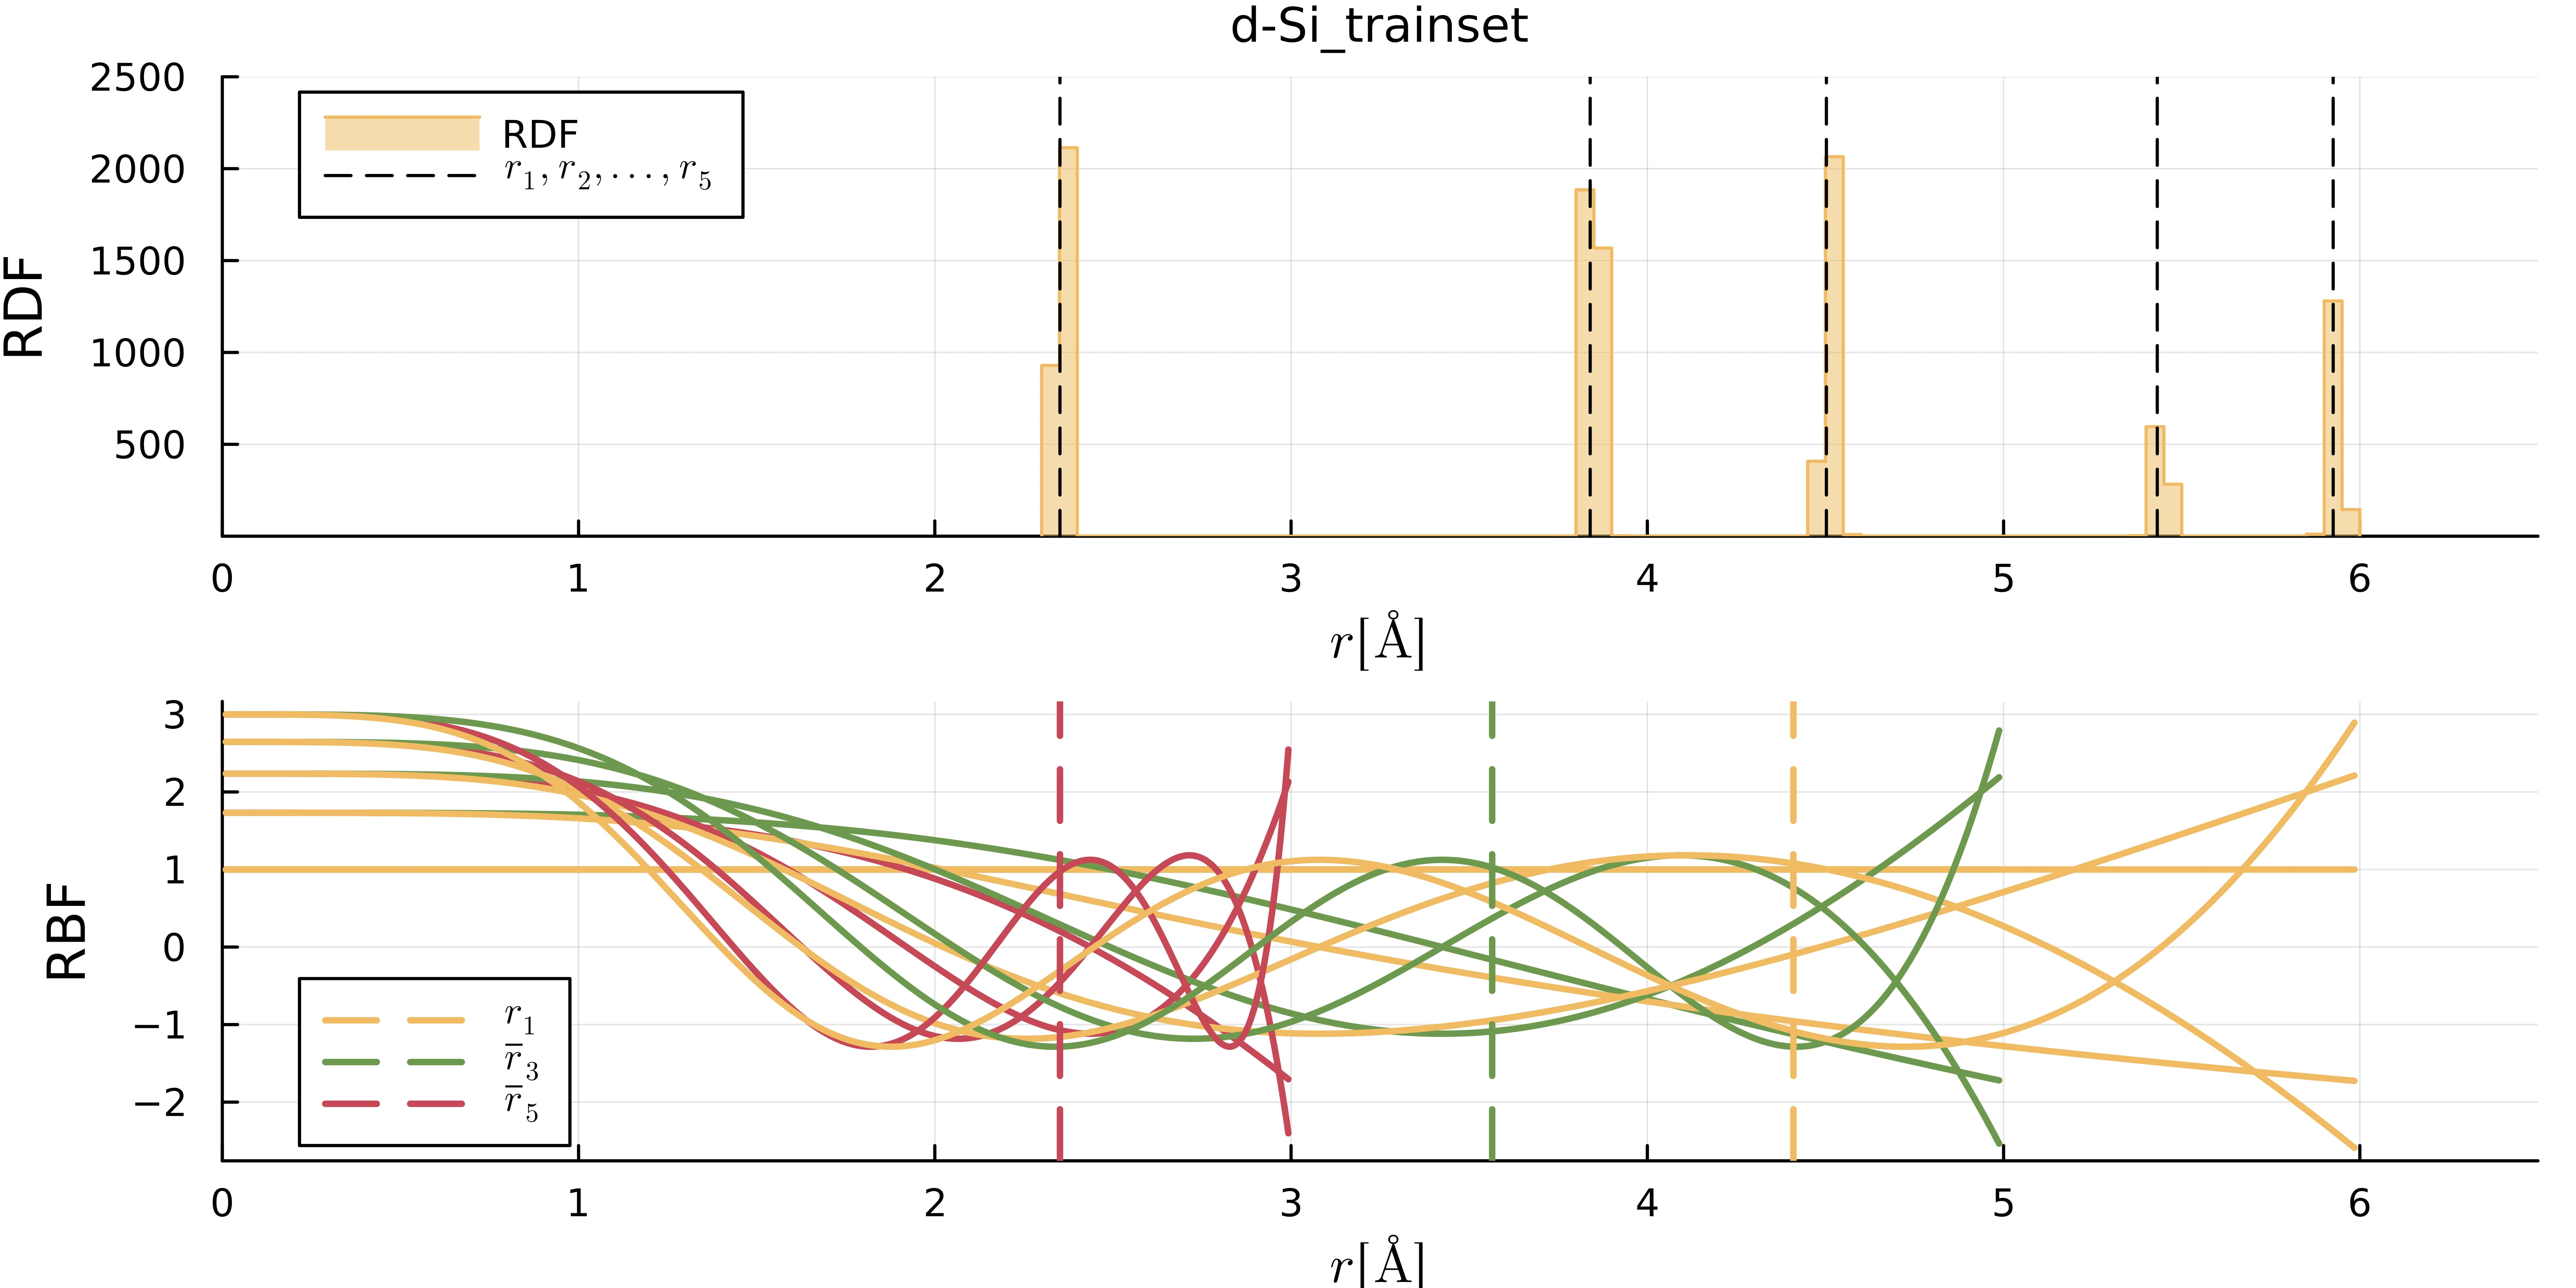
\includegraphics[width=1.0\textwidth]{Figure/Chapter 3/ACE/_RDF_RBF_Si.jpg}
\caption{\label{fig:3.10} 
Radial distribution function (RDF) and radial basis functions (RBF) for the d-\textbf{Si} training set. 
    }
\end{figure*}

Let us consider the top panel of Figure~\ref{fig:3.10}, which shows the RDF histogram of the input d-\textbf{Si} dataset, with dashed black lines indicating the set of equilibrium bond lengths of silicon (\( r_1,\, r_2,\, \dots,\, r_5 \)). The bottom panel illustrates the possible choices of radial basis sets (centred at the average of these distances within the cutoff radiuis 3~\AA~(red), 5~\AA~(green), 6~\AA~(yellow)), extracted from the code shown in Figure~\ref{fig:3.9}.
We construct three sets of radial basis functions, shown in red, green, and yellow, designed to cover the first peak, the first three peaks, and all peaks in the RDF, respectively.
These three sets are characterised by different cutoff radii and corresponding average equilibrium bond lengths, i.e., \(\{3~\text{\AA},\, r_1\}\), \(\{5~\text{\AA},\, \overline{r}_3\}\), and \(\{6~\text{\AA},\, \overline{r}_5\}\), where \(\overline{r}_3\) and \(\overline{r}_5\) denote the averages of \(\{r_1,\, r_2,\, r_3\}\) and \(\{r_1,\, r_2,\, \dots,\, r_5\}\), respectively.

After obtaining the appropriate radial basis set for the individual centred atom, we can then form the descriptor of the $N$-atom structure by concatenating the many-body product basis for all atoms in the structure.
This total structure descriptor is expressed as
\begin{equation} \label{equ:3.25}
    \mathbf{B}_{\text{tot}} = 
    \begin{bmatrix}
        \mathbf{B}_{1} &
        \mathbf{B}_{2} &
        &\cdots&
        \mathbf{B}_{N}
    \end{bmatrix}^{\text{T}},
\end{equation}
where each $\mathbf{B}_{i}$ is defined in Equation \eqref{equ:3.24}.
Therefore, the size of the full descriptor \(\mathbf{B}_{\text{tot}}\) is given by the size of the ACE model basis, \(\text{dim}(\mathbf{B}_i)\), multiplied by the number of atoms \(N\) in the structure. For example, using the ACE basis constructed by the code in Figure~\ref{fig:3.9}, the descriptor size for a \(2\times2\times2\) d-\textbf{Si} supercell is \(12 \times 16 = 192\) degrees of freedom.
\begin{figure*}[t]
  \centering
  \begin{lstlisting}[language=Julia]
model = (*@\textcolor{bEpic}{acemodel}@*)(elements = [(*@\textcolor{rEpic}{:Pb}@*), (*@\textcolor{rEpic}{:Te}@*),],
	order = 2,                 #3-body order
	totaldegree = 5,
        r0 = (rnn((*@\textcolor{rEpic}{:Pb}@*))+rnn((*@\textcolor{rEpic}{:Te}@*)))/2,
	rcut = 6.5,
	pair_transform = ((*@\textcolor{rEpic}{:agnesi}@*), p = 1, q = 4),
	pair_envelope = ((*@\textcolor{rEpic}{:r}@*), 2, 2)
    )
	@show length(model.basis)
(*@\textcolor{bEpic}{> length(model.basis)}@*) = 65
  \end{lstlisting}
  \caption{\label{fig:3.11} Construction of a 3-body order ACE descriptor for a \textbf{PbTe}-structure using a total degree constraint of 5, an Agnesi radial transform, and a smooth polynomial envelope.}
\end{figure*}

We also investigate the construction of ACE descriptors for a \textbf{PbTe} structure as an example of a multi-element system. The many-body product basis set can be generated using the code shown in Figure~\ref{fig:3.11}, which follows a similar procedure to the d-\textbf{Si} case, with the change for accounting for the two input elements and the average equilibrium bond length of the \textbf{Pb–Te} pair.

The hyperparameters \texttt{r0}, \texttt{rcut}, \texttt{pair\_transform}, and \texttt{pair\_envelope} are determined by analysing the RDFs and RBFs of the input \textbf{PbTe} structure, as illustrated in Figure~\ref{fig:3.12}. Since \textbf{PbTe} is a two-element system, it is necessary to consider the radial distributions between \textbf{Pb–Pb}, \textbf{Pb–Te}, and \textbf{Te–Te} atom pairs, which are shown as yellow, green, and red lines, respectively, in the RDF histogram in the top panel.

The \texttt{r0} parameter is selected as the average position of the first three RDF peaks, as the fourth peak, associated with the \textbf{Pb–Te} bond length, is relatively small compared to the others. The \texttt{rcut} parameter is chosen to cover the fourth peak, while \texttt{pair\_transform} and \texttt{pair\_envelope} are employed identically to the d-\textbf{Si} case. The resulting radial basis functions (RBFs) extracted from the ACE model with these parameters are shown in the bottom panel of Figure~\ref{fig:3.12}.

\begin{figure*}[t]
\centering
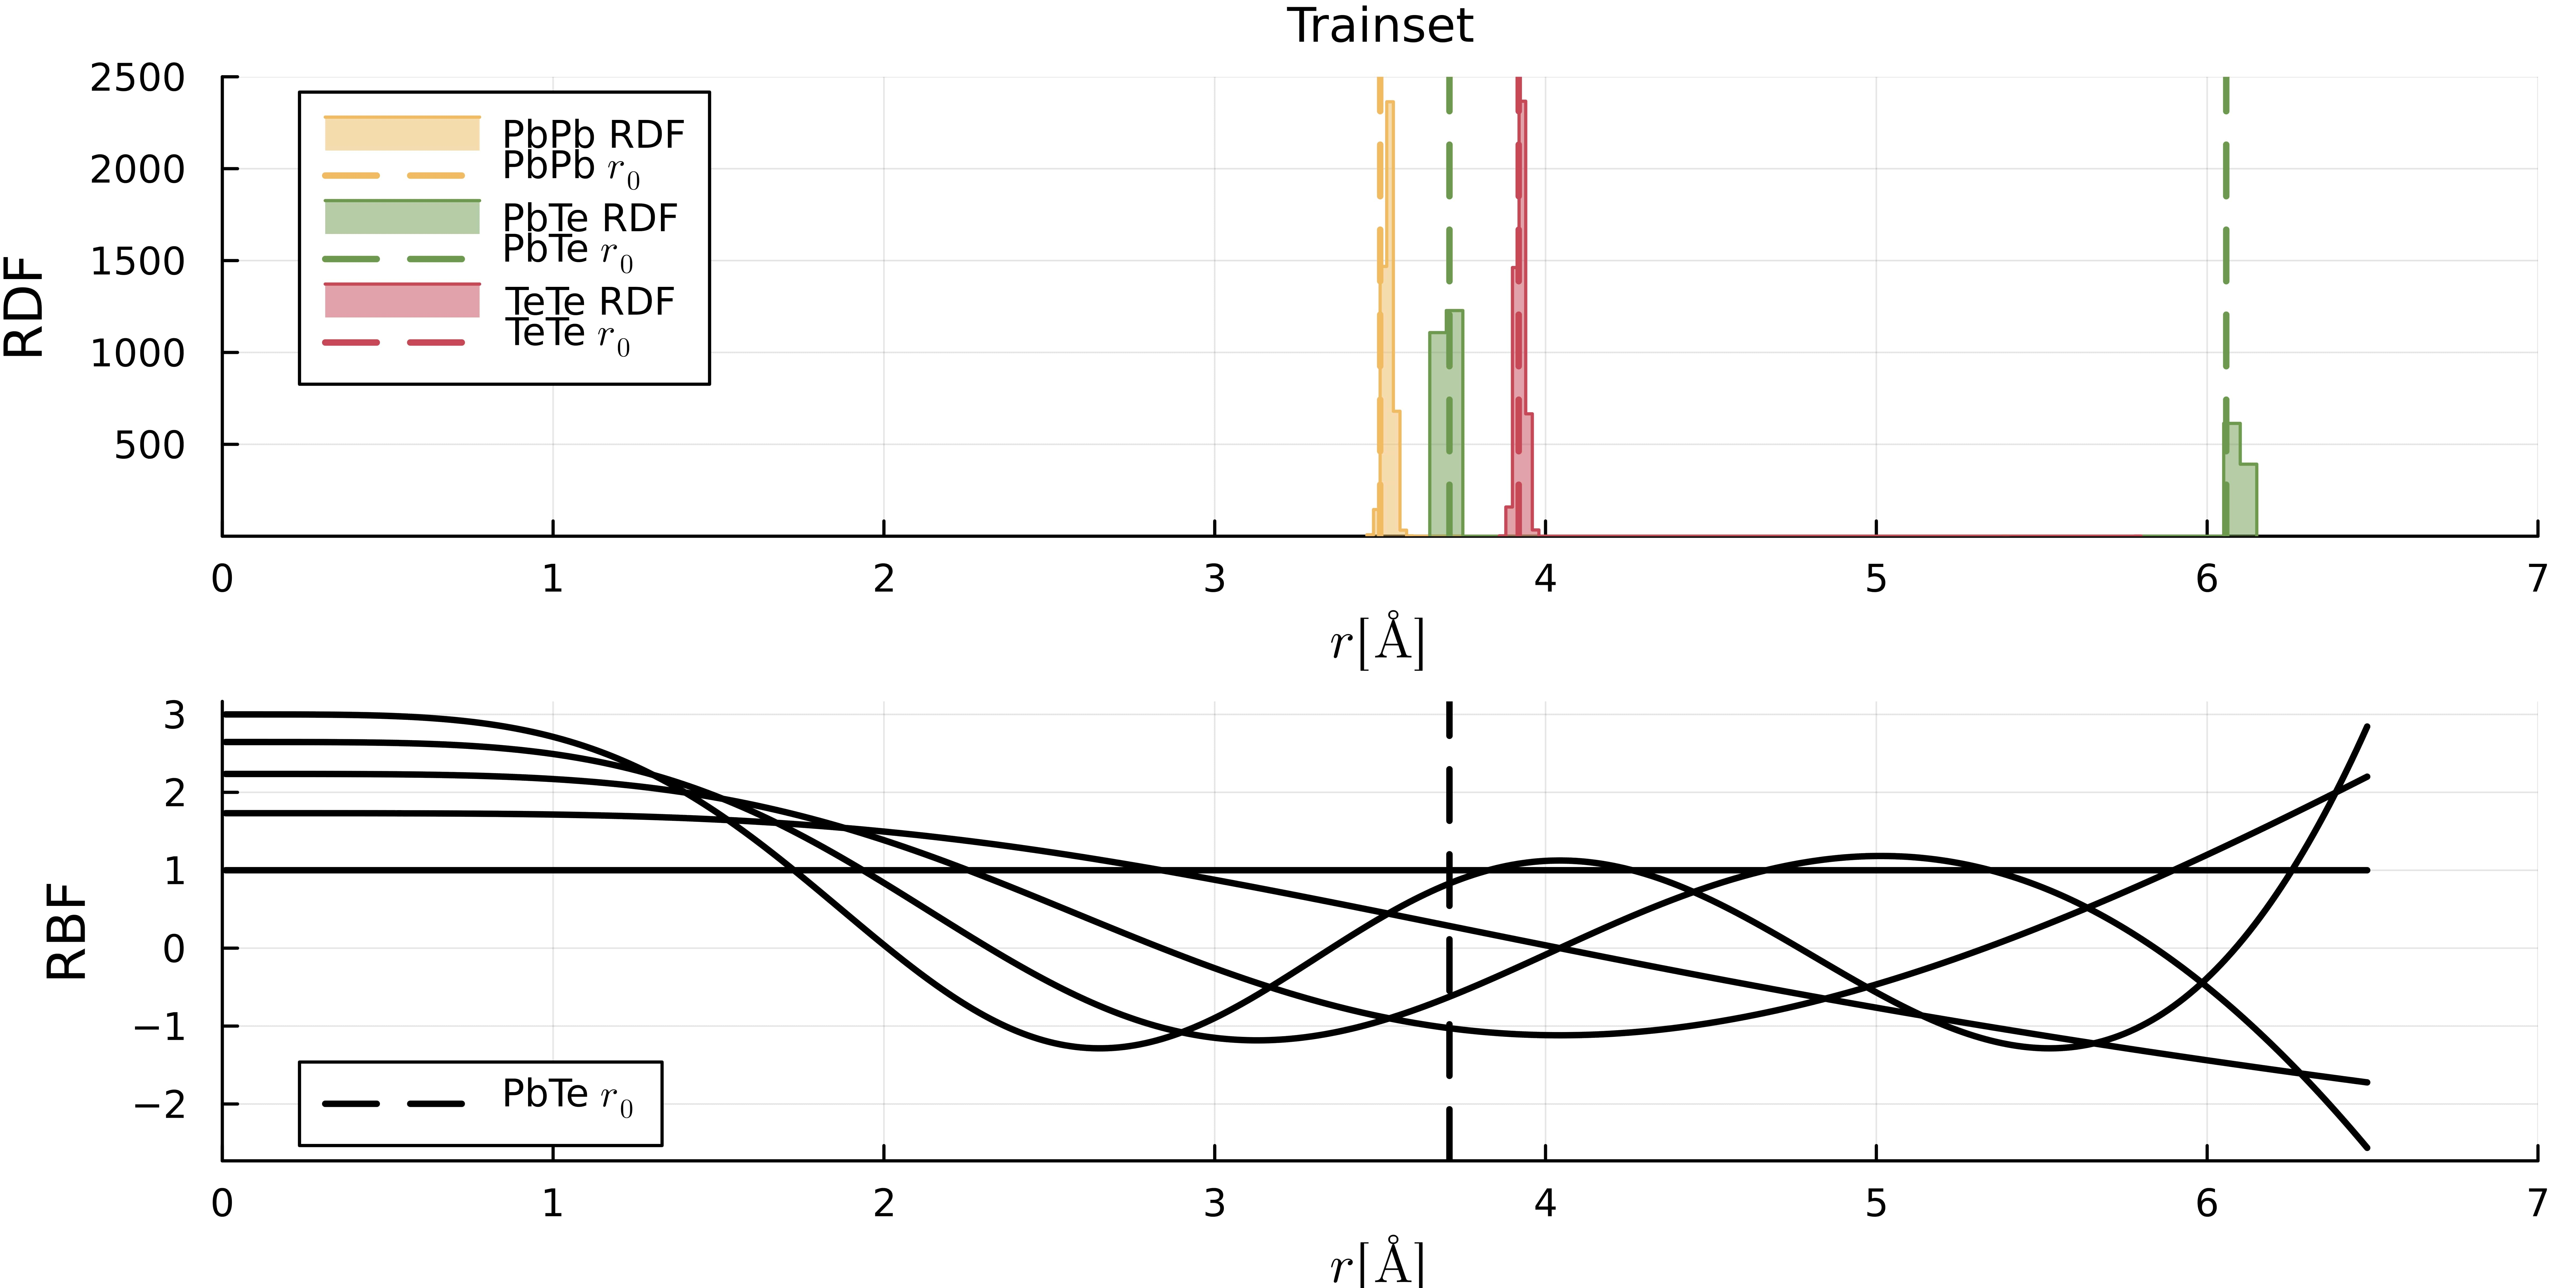
\includegraphics[width=1.0\textwidth]{Figure/Chapter 3/ACE/_RDF_RBF_PbTe.jpg}
\caption{\label{fig:3.12} 
Radial distribution function (RDF) and radial basis functions (RBF) for the \textbf{PbTe} training set. 
%(Top) yellow, green, and red lines RDF histograms with the corresponding dashed yellow, green, and red lines indicating equilibrium bond-lengths for \textbf{Pb-Pb}, \textbf{Pb-Te}, and \textbf{Te-Te}, respectively.
%(Bottom) Radial basis functions centred at the \textbf{Pb-Te} equilibrium bond length within the cutoff radiuis 6.5~\AA, capturing local atomic environments.
    }
\end{figure*}
To construct the full descriptor \(\mathbf{B}_{\text{tot}}\) for the \textbf{PbTe} structure, we can now perform Equation~\eqref{equ:3.25}, resulting in a \(65 \times 16 = 1040\)-dimensional feature vector.
This descriptor size of 1040 degrees of freedom also applies to other two-element systems, such as \textbf{NaCl}, \textbf{GaAs}, and \textbf{CdTe}, when using the same hyperparameter settings.

However, we observe that incorporating ACE descriptors directly into our differentiable GP model may not be sufficiently efficient, as the size of the ACE descriptors is significantly larger than that of the Cartesian and phonon descriptors. 
This increased descriptor size impacts both the computational cost and memory requirements for calculating higher-order derivatives with the current version of automatic differentiation.
Therefore, instead of using ACE descriptors directly in the GP model, we propose to incorporate the ACE framework in an alternative way, namely for data generation and active learning, which will be discussed in the next subsection.

\subsection{ACE fitting} \label{subsec:3.3.2}

\begin{figure*}[t]\centering
\begin{subfigure}{.5\textwidth}
  \centering
  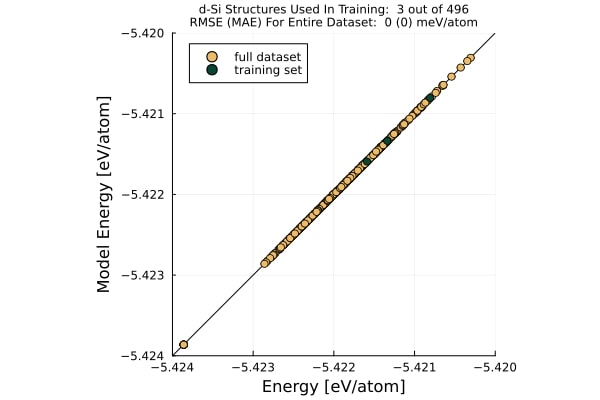
\includegraphics[width=1\linewidth,height=\textheight,keepaspectratio]{Figure/Chapter 3/ACE/fitting_Si_.jpg}
  \caption{}
\end{subfigure}%
\begin{subfigure}{.5\textwidth}
  \centering
  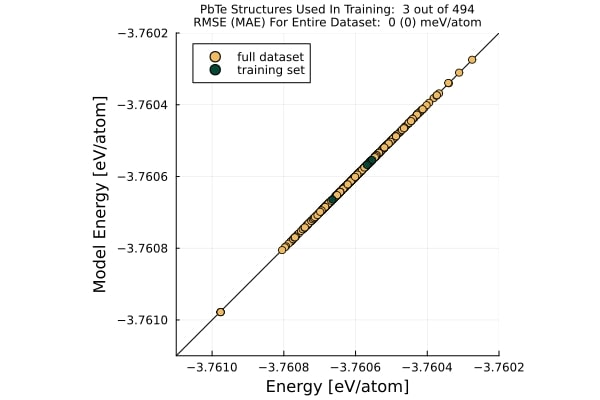
\includegraphics[width=1\linewidth,height=\textheight,keepaspectratio]{Figure/Chapter 3/ACE/fitting_PbTe.jpg}
  \caption{}
\end{subfigure}
\caption{
    \label{fig:3.13}
    Panels (a) and (b) show  the ACE-fitted potentials for an input d-\textbf{Si} and \textbf{PbTe} training data point (blue) alongside the corresponding target energies (yellow).
}
\end{figure*}

In this section, we discuss an alternative approach for incorporating the ACE framework into our differentiable GP model. To generate datasets efficiently, we use the \textsc{ACEpotentials} instead of ACE descriptors as inputs.

The \textsc{ACEpotentials} enables highly accurate energy fitting for both d-\textbf{Si} and \textbf{PbTe} structures.
Using the ACE model settings shown in Figures~\ref{fig:3.9} and~\ref{fig:3.11}, we train the ACE model with only three data points obtained from DFT calculations\footnote{The DFT calculations are performed using \textsc{VASP}, with convergence settings detailed in Subsection~\ref{subsec:3.1.2}.}. 

With the minimal training set, the ACE model achieves excellent predictive accuracy: it recovers all 500 energy values with RMSEs (MAEs) of \(2.37 (1.84)~\mu\text{eV}\)/atom for the d-\textbf{Si} structure and \(136.18 (6.68)~\mu\text{eV}\)/atom for the \textbf{PbTe} structure, as shown in Figure~\ref{fig:3.13}. The RMSEs (MAEs) of the predicted forces are similarly low, at \(0.89 (0.68) ~\text{meV}/\text{\AA}\) for d-\textbf{Si} and \(0.11 (0.09) ~\text{meV}/\text{\AA}\) for \textbf{PbTe}.

The strong predictive performance of the ACE model enables efficient generation of energies and forces for new data points, which can be used to further train our GP model. These new configurations, denoted as \(\{\mathbf{x}'_{1},\;\mathbf{x}'_{2},\;\dots,\;\mathbf{x}'_{n}\}\), can initially be sampled from a normal distribution around the equilibrium structure.

We offer two approches to benefit from using these Linear ACE data. One is directly doing finite different methods to calculate force constants for phonon calculations. This will be discussed in the next subsection. Another is doing Active learning on top of GPFC models which the guidance is provide in subsection \ref{subsec:3.3.4}.  

\subsection{Phonons from Linear ACE data} \label{subsec:3.3.3}

\begin{figure*}[t]\centering
\begin{subfigure}{.5\textwidth}
  \centering
  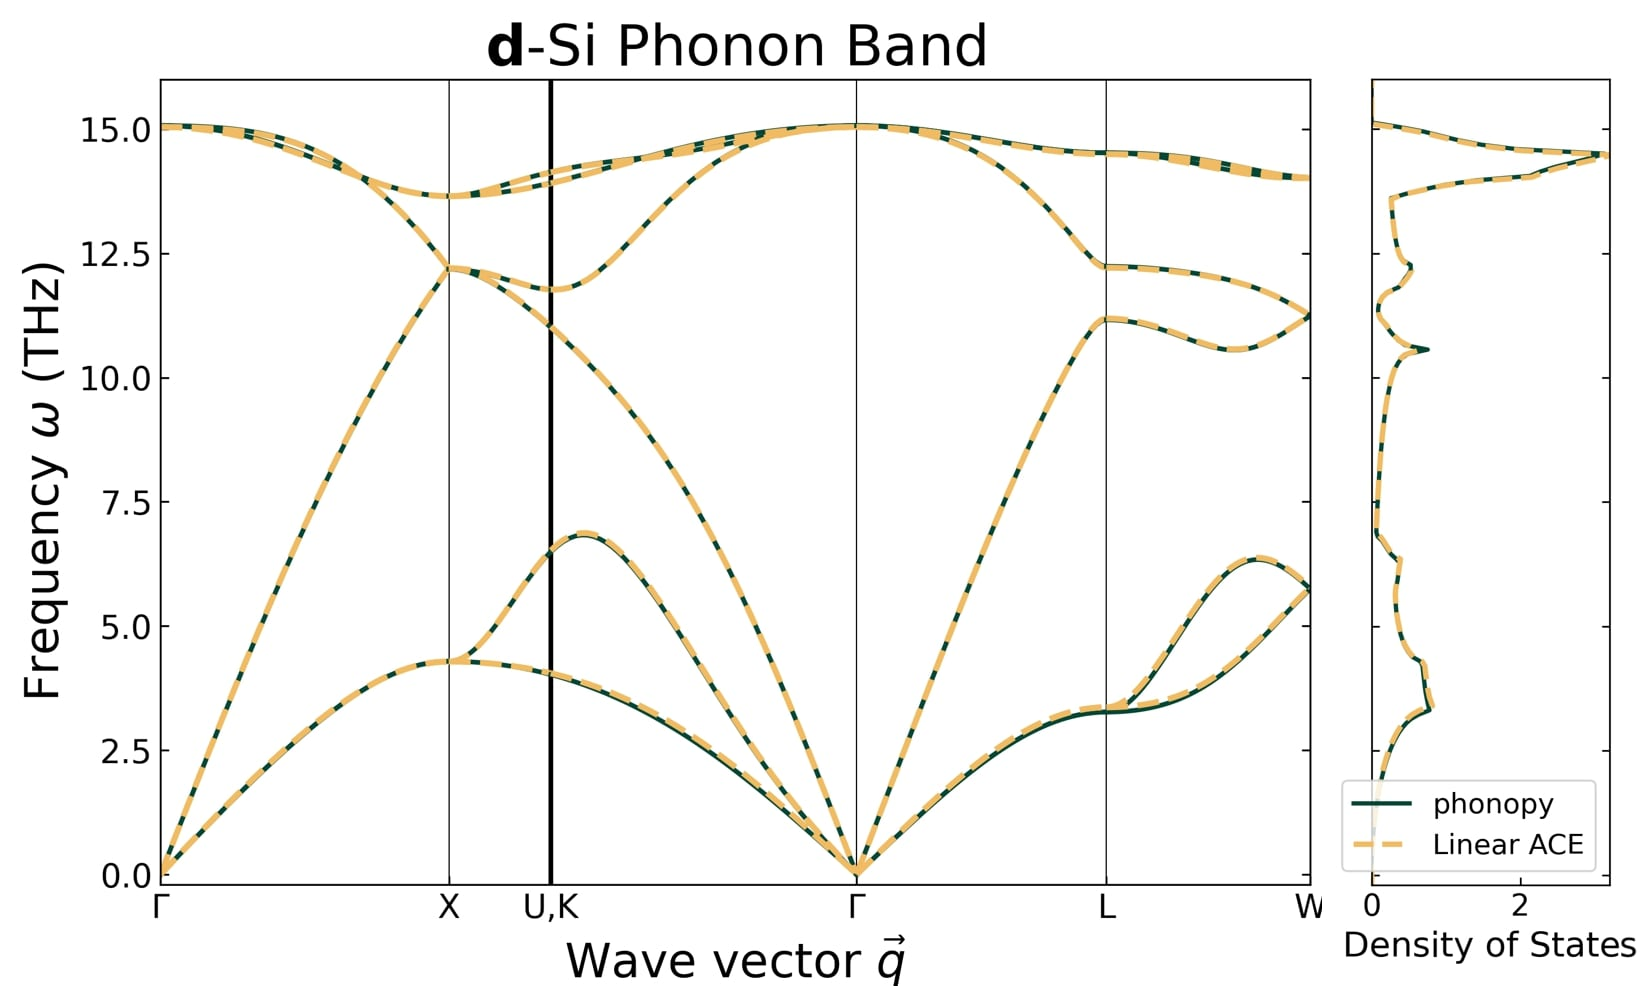
\includegraphics[width=1\linewidth,height=\textheight,keepaspectratio]{Figure/Chapter 3/ACE/d-Si.jpg}
  \caption{}
\end{subfigure}%
\begin{subfigure}{.5\textwidth}
  \centering
  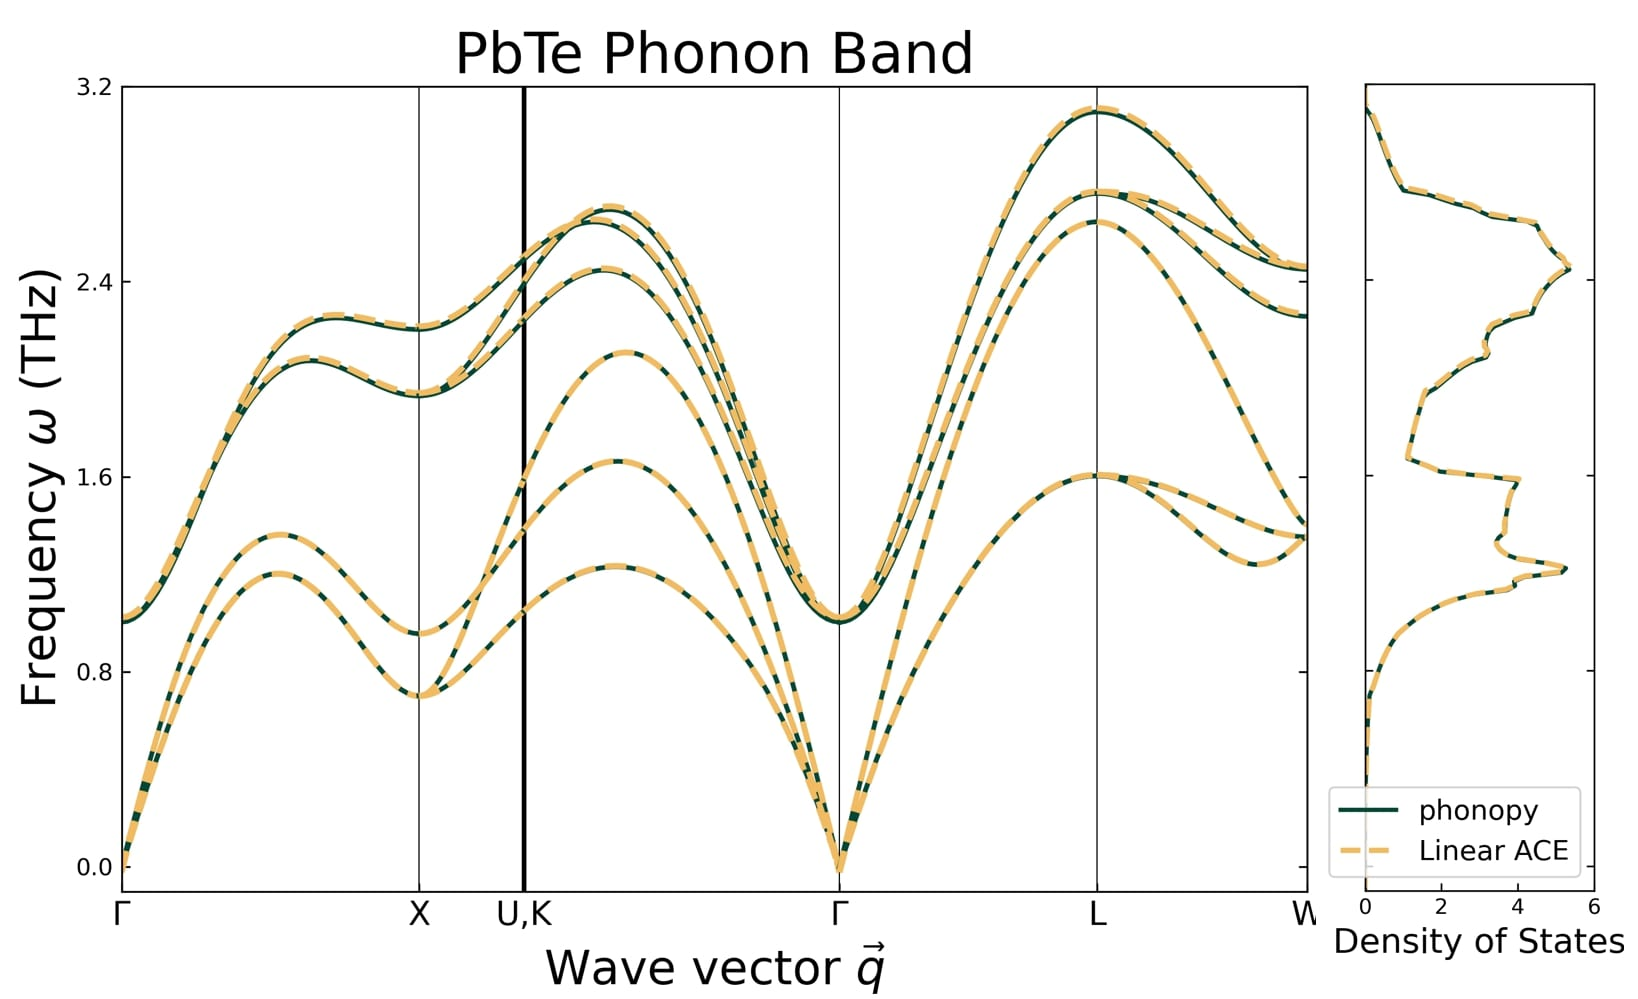
\includegraphics[width=1\linewidth,height=\textheight,keepaspectratio]{Figure/Chapter 3/ACE/PbTe.jpg}
  \caption{}
\end{subfigure}
\caption{
    \label{fig:3.13.1}
    Panels (a) and (b) show the phonon band structures and density of states for d-\textbf{Si} and \textbf{PbTe}, respectively. 
}
\end{figure*}

The highly accurate forces obtained from the linear ACE model enable accurate phonon calculations using standard approaches such as Finite Difference Methods (FDM).

To evaluate the fitting results against our model, it is necessary to disregard the crystal symmetry (i.e., deactivate the symmetry in \textsc{phonopy}).
We compute the harmonic force constants using the data point number of $6N$, where $N$ indicates the number of atoms in the system as mentioned in section \ref{subsec:2.1.1}.  For a \(2\times2\times2\) diamond-structured silicon and a \(2\times2\times2\) lead telluride, the symmetry-breaking force distribution matrices necessitate 96 data points (16 atoms per system). 

The results are illustrated in figure~\ref{fig:3.13.1}.  Their RMSEs are roughly 1.01% for d-Si and 1.52% for PbTe, both of which are significantly lower than GPFC.

This shows that the Linear ACE model is potentially powerful for using generating dataset for the study of phonons. For the future work, we will propose this to capture the anharmonic phonons.

\subsection{Active learning with Linear ACE data} \label{subsec:3.3.4}
Moreover, we can apply an active learning strategy \cite{Hoang2014,Khatamsaz2023,Ghorbani2024,https://doi.org/10.48550/arxiv.1911.09946} to select the next data points by maximising the predictive variance of the Gaussian process force constants. The predictive variance of the GPFC2 model is defined as

\begin{equation} \label{equ:3.26}
\begin{split}
\Sigma^{(2)}(\mathbf{x}^{*}) ={}& 
\left[
    (\nabla_{\mathbf{x}^{*}})^2 (\nabla_{\mathbf{x}})^2 k
\right]_{\mathbf{x}^{*},\;\mathbf{x}^{*}}\\
&- 
\begin{bmatrix}
    (\nabla_{\mathbf{x}^{*}})^2 k &
    (\nabla_{\mathbf{x}^{*}})^2 \nabla_{\mathbf{x}} k
\end{bmatrix}_{\mathbf{x}^{*},\;\mathbf{x}}
\cdot \mathcal{K}^{-1}_{\mathbf{x},\, \mathbf{x}}
\cdot
\begin{bmatrix}
    (\nabla_{\mathbf{x}^{*}})^2 k\\
    (\nabla_{\mathbf{x}^{*}})^2 \nabla_{\mathbf{x}} k
\end{bmatrix}_{\mathbf{x},\;\mathbf{x}^{*}},
\end{split}
\end{equation}

which corresponds to the predictive mean of GPFC2s given in Equation~\eqref{equ:3.7} and is analogous to the predictive variance of the energy in a differentiable GP model, as defined in Equation~\eqref{equ:2.45}.
The next data point can be selected by maximising the predictive variance according to the following expression:

\begin{tcolorbox}[
    ams equation,
    title=Maximization of Predictive GPFC2 Variance,
    colframe=bEpic,
    coltitle=white,
]
\label{equ:3.27}
\begin{split}
\mathbf{x}'_{\text{next}} =
\arg\max_{\mathbf{x}^{*}}\; \Sigma^{(2)}(\mathbf{x}^{*}),
\end{split}
\end{tcolorbox}

where \(\Sigma^{(2)}(\mathbf{x}^{*})\) is defined in Equation~\eqref{equ:3.26}. Finding \(\mathbf{x}'_{\text{next}}\) requires differentiating \(\Sigma^{(2)}(\mathbf{x}^{*})\) with respect to \(\mathbf{x}^{*}\), which in turn demands evaluation of up to the fifth-order derivatives of the kernel function.

Meanwhile, active learning for the GPFC3 model would require constructing an analogous expression for the predictive variance of GPFC3, followed by maximisation to select the next data point. In this case, kernel derivatives up to the seventh order would be required.

At present, we have implemented only the random sampling method in our model. Full implementation of the active learning strategy remains challenging, as performing high-order automatic differentiation leads to substantial memory demands. However, analytic expressions for arbitrary-order derivatives of the radial basis function (RBF) kernel are provided in Appendix~\ref{sec:A.1}, which may facilitate future improvements.


%\begin{tcolorbox}[
%    ams equation,
%    title=Predictive variance of GPFC3,
%    %colback=blue!5,
%    colframe=bEpic,
%    %colframe=blue!75!black,
%    coltitle=white,
%    %fontupper=\color{blue}  % << changes font color inside the box
%]
%\label{equ:3.27}
%\begin{split}
%    \Sigma^{(3)}(\mathbf{x}^{*}) =& \begin{bmatrix}
%          (\nabla_{\mathbf{x}^{*}})^3 (\nabla_{\mathbf{x}})^3 k
%    \end{bmatrix}_{\textbf{x}^{*},\;\textbf{x}^{*}}\\ &+
%    \begin{bmatrix}
%          (\nabla_{\mathbf{x}^{*}})^3 k &
%          (\nabla_{\mathbf{x}^{*}})^3 \nabla_{\mathbf{x}} k
%    \end{bmatrix}_{\textbf{x},\;\textbf{x}^{*}}
%        \cdot \mathcal{K}^{-1}_{\mathbf{x},\: \mathbf{x}}
%        \cdot
%        \begin{bmatrix}
%              (\nabla_{\mathbf{x}^{*}})^3 k\\
%              (\nabla_{\mathbf{x}^{*}})^3 \nabla_{\mathbf{x}} k
%        \end{bmatrix}_{\textbf{x},\;\textbf{x}^{*}},
%\end{split}
%\end{tcolorbox}

\section{Conclusion and Future work} \label{sec:3.4}

We developed a differentiable Gaussian process (GP) model for predicting harmonic (second-order) and cubic anharmonic (third-order) force constants. Our approach, which is incorporated into the \textsc{GPFC.jl} package, uses higher-order kernel derivatives to predict force constants directly from density functional theory (DFT)-calculated energies and forces.

Initially, we employed Cartesian descriptors, validating the model by comparing the predicted GPFC2 and GPFC3 tensors against finite displacement method (FDM) results for several representative materials. Accurate phonon properties, including band structures, density of states, phonon lifetimes, and lattice thermal conductivities, were obtained from the GPFC predictions with excellent agreement relative to traditional FDM approaches.

To improve model efficiency, we introduced phonon-mode descriptors, which inherently impose system symmetries and reduce the dimensionality of the learning problem. Using phonon descriptors significantly decreased the number of training data required, particularly for GPFC2 predictions, while maintaining or improving model accuracy.

We also outlined procedures for transforming phonon-based force constants back into the Cartesian basis, necessary for full Brillouin zone sampling and thermal property calculations. Although our current implementation is restricted to real-valued descriptors (thus, the $\Gamma$-point), we proposed strategies for handling complex descriptors in future extensions.

Furthermore, we investigated how the Atomic Cluster Expansion (ACE) framework might be integrated. While direct incorporation of ACE descriptors into our GP model proved inefficient due to large descriptor sizes, we proposed and tested an alternative: using ACE models for rapid and accurate data generation. With minimal DFT training, ACE potentials were able to reproduce reference datasets with very low errors, making them ideal for augmenting GPFC training through either random sampling or active learning.

Finally, we outlined an active learning strategy based on maximising the predictive variance of the GPFCs to help guide the selection of new training data. The full implementation of the active learning procedure is still challenging due to the memory demands of high-order derivatives, but the analytic expressions provided in the Appendices pave the way for future work.

In summary, this study introduces a flexible and powerful framework for learning force constants with differentiable Gaussian processes. 
By improving both accuracy and data efficiency, it creates new possibilities for modelling lattice thermal properties and anharmonic phonons in complex materials.
